% TEX-root = ../main.tex
\chapter{总结与展望}
本章将总结本文现有的工作,并对未来的可能的研究方向进行展望。
\section{总结}
当前虚拟现实、自由视点视频、街景地图等领域对新视图合成存在大量需求,通过对现有的相关系统进行调研发现存在以下问题:1) 当前市场上的三维渲染的软件难以根据稀疏视图,在任意视角下渲染出高质量的新视图;
2) 目前的三维渲染系统大都需要根据深度信息进行三维建模,这需要使用 RGBD 相机,对硬件设备要求较高;
3) 目前市场上还没有直接可应用的面向快速新视图合成的交互系统;4) 现有的新视图合成模型需要在空间内进行大量采样,计算时间成本较高,难以完成 PC 端的交互需求。在这样的背景下,本文结合 NeRF 的技术以及查询表缓存加速的相关技术实现了快速合成新视图的神经辐射场渲染具体方法,并设计和实现了一个快速新视图合成的系统,完成了 PC 客户端的相关应用。

本文的主要工作与贡献如下:

\begin{enumerate}
	\item [1)] 本文基于 NeRF 预训练的网络预测的体密度信息构建出一个可以表征在物体内外的查询表结构,这一方面直接减少了查询表的尺寸,另一方面该查询表可以直接为空间内任意一点提供 NeRF 网络中间层的特征,这加快了神经网络的正向传播速度。
	\item [2)] 在缓存了上述查询表的基础上,本文改进了 NeRF 的采样过程,通过查询表找到光线上离物体表面最近的内点,使得 NeRF 可以仅在此点附近进行采样,从而不必再使用两个网络,这显著加速了 NeRF。
	\item [3)] 为了补偿查询表分辨率不够带来的精度损失,本文对 F-NeRF 进行再训练,将渲染质量提升到原 NeRF 的水平。
	\item [4)] 本文在公开的数据集上做了大量对比验证实验。在公开合成数据集 Synthetic-NeRF 和真实场景数据集 LLFF-NeRF 上,与 NeRF 相比,我们提出的 F-NeRF 方法分别加速 3.2 倍和 3.4倍。 
	\item [5)] 本文设计并实现了基于 NeRF 的快速新视图合成的系统,完成了相应的 PC 端的应用,并对该系统进行了详细的需求分析以及架构设计,最后将本文的方法实现并部署到了 PC 端,经过详细地测试,该系统满足实际应用需求。
\end{enumerate}


\section{展望}
本文实现的基于神经辐射场的快速新视图合成系统保留了人机交互的自然、简洁等优点,并保证了交互的一致性与实时性,具有一定的应用前景。但系统仍存在一些值得思考与完善的地方:
\begin{enumerate}
	\item 本文基于 NeRF 改进的快速新视图合成方法本质还是假设输入图像为静态图像,然而在真实场景里,这是很难做到的。因此在未来希望通过改进算法使得系统输入动态图像也可以合成较高质量的视图。
	\item 目前本系统的方法使用的查询表提取到的物体几何信息不够准确,这是因为缓存的点过于稀疏,对于空洞较多的场景渲染出的新视图质量不够好。因此在未来可以借助 mesh 缓存场景的几何信息,使用 ray tracing 的方法去找到物体表面,从而可以更好地优化采样点的位置。
	\item 由于测试的时候还是使用了神经网络,因此本系统还不足以做到实时的合成新视图。因此未来可以转换思路,从缓存网络参数到直接缓存输出的颜色和体密度,这样可以让测试的过程与神经网络解耦,从而地合成新视图。
\end{enumerate}

















% \begin{enumerate}
%     \item \texttt{sysusetup.tex}: 填写标题、作者、导师、学位名称等信息。
%     \item \texttt{data/abstract.tex}: 填写中英文摘要。
%     \item \texttt{data/denotation.tex}: 填写符号与缩略语,注意按音序排序。
%     \item \texttt{data/chapxx.tex}: 各章内容,如有章节增删请在\texttt{main.tex}中修改相关记录。
%     \item \texttt{data/appendix.tex}: 附录。
%     \item \texttt{data/works.tex}: 学术成果。
%     \item \texttt{data/acknowledgements.tex}: 致谢。
%     \item \texttt{ref/refs.bib}: 引文数据库。
%     \item \texttt{main.tex}: 主文件,用于控制文档选项(字体,学位类别):
%     \begin{enumerate}
%         \item 学术硕士: \verb|\documentclass[degree=master]{sysuthesis}|;
%         \item 专业硕士: \verb|\documentclass[degree=master,degree-type=professional]{sysuthesis}|;
%         \item 博士: \verb|\documentclass[degree=doctor]{sysuthesis}|。
%     \end{enumerate}
%     指定论文要包括的部分,如摘要、目录、正文各章节、附录、引文数据库等等。
%     (注意插入每章内容之后要加 \verb|\cleardoublepage| 以保证在打印版中各章都从右边开始):
%     \begin{verbatim}
%     % !TeX root = ../main.tex

\chapter{绪论}

本章作为绪论主要介绍了神经辐射场中新视图合成加速问题的背景与意义,分析了目前相关技术与算法的发展现状以及相关系统存在的问题,阐述了解决该问题的必要性,然后总结了本文的主要工作与贡献,最后概述了本文的章节结构。

\section{研究背景与意义}
近年来,随着深度学习与计算机视觉的飞速发展,人类的生活愈来愈趋向智能化。在以前,人们必须通过行万里路来了解这个世界,但是现在,可以通过全景地图几乎全方位地去观察一个未知的地方,甚至是通过虚拟现实,增强现实等形式沉浸式地以任意的角度呈现出场景或者物体。新视图合成技术可以支持以上应用场景,可以通过已有的图像去合成新视角下的图像。

新视图合成任务\cite{chen1993view}作为计算机视觉和计算机图形学的交叉领域任务,有着极其广阔的应用前景,一直是学术界和工业界的热门研究问题。新视图合成任务具体是,通过给定的已知视角下观测到的图像,去合成新视角下的图像。图~\ref{fig:FreeViewSynthesis} 给出了新视图合成任务的示意图。

\begin{figure}[tbhp]
    \centering
    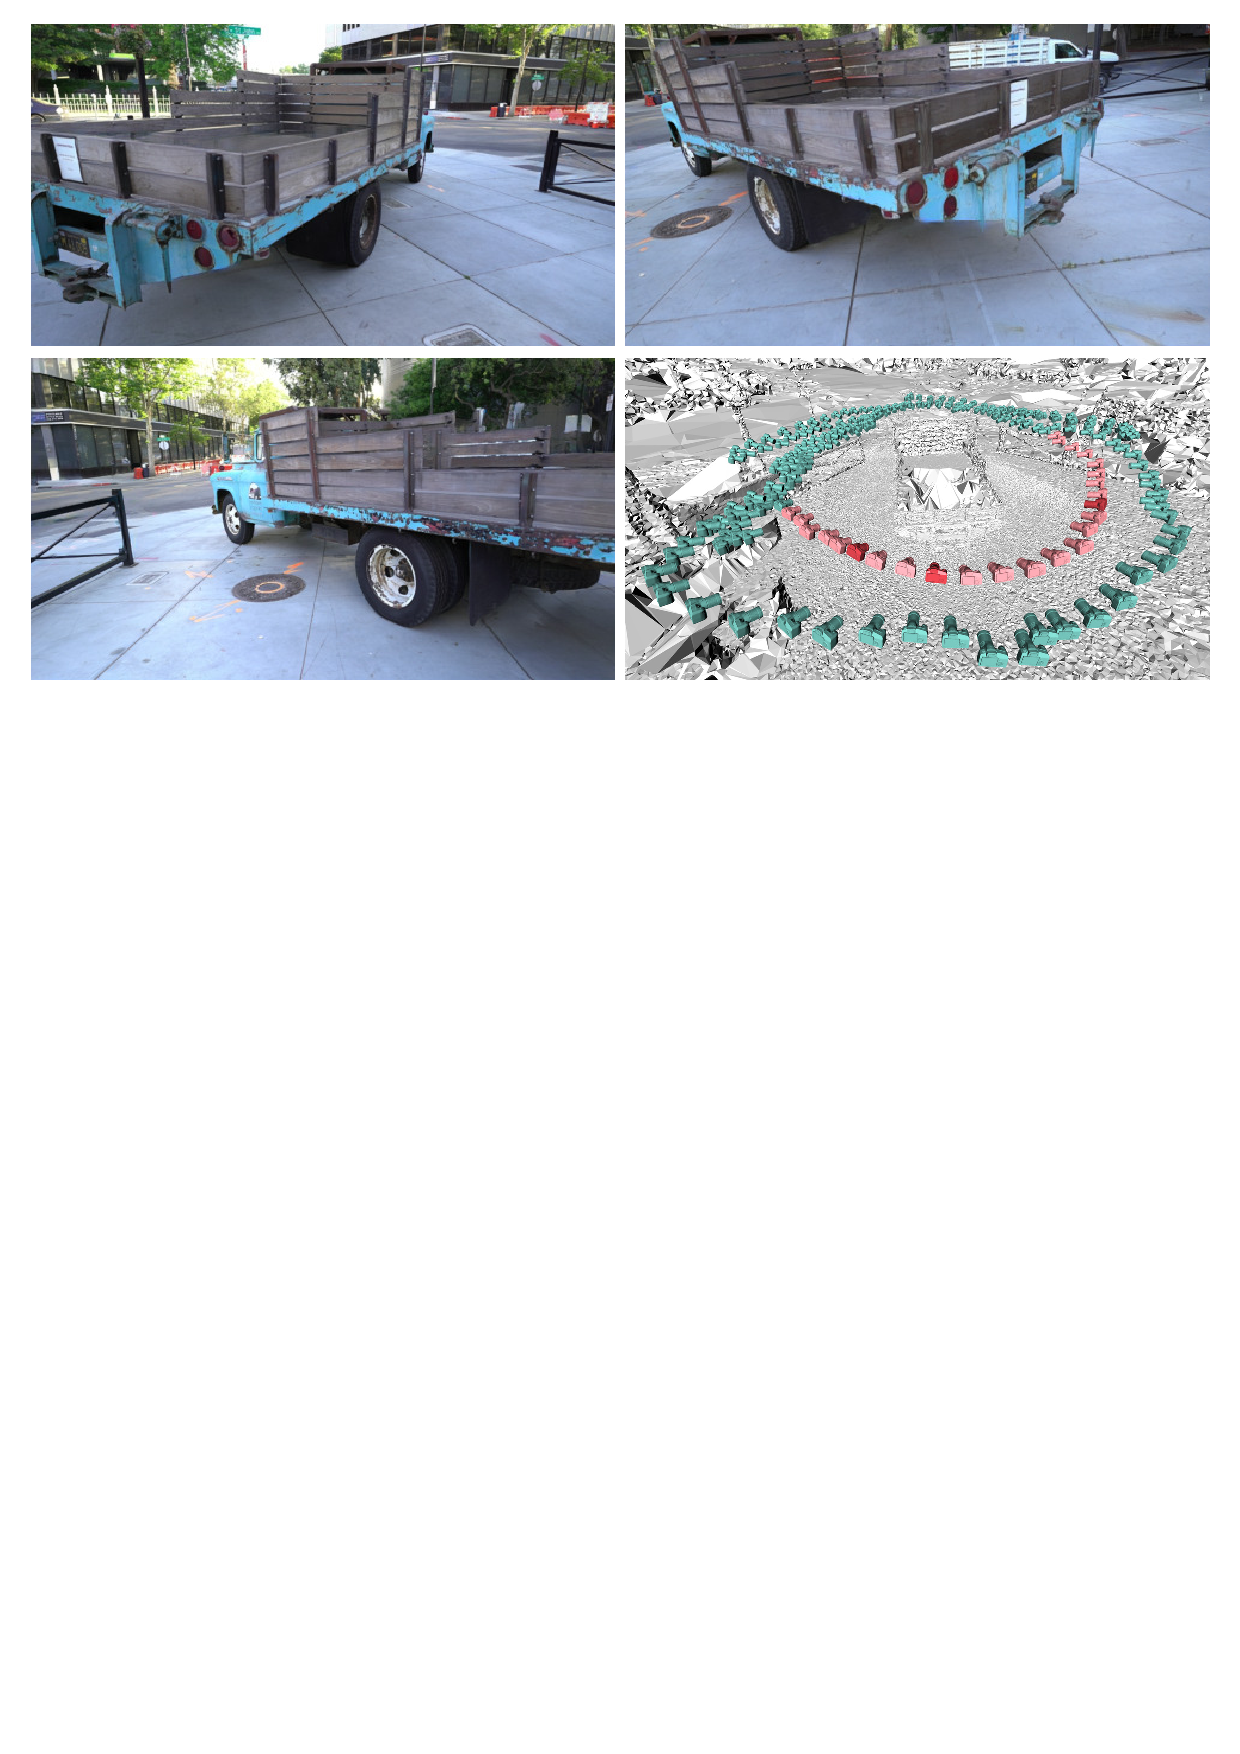
\includegraphics[width=0.95\textwidth]{figures/FreeViewSynthesis.pdf}
    \caption{新视图合成的示意图\cite{riegler2020free}。前三张图是合成的新视图,最后一张图阐明了绿色相机位姿下的图像作为输入,推理红色相机位姿的新视图。}
    \label{fig:FreeViewSynthesis}
\end{figure}
\newpage

根据前期调研,新视图合成技术有着广泛的应用前景,市场需求庞大,急需可快速合成高质量新视图的系统。而在实际应用中,限于应用需求和经济成本等因素的考量,市场上的大多产品仍存在着许多问题,比如无法在任意角度合成高质量图像,另外渲染新视图的时间过长,这些都严重影响了用户体验。而本身,三维场景具有一定复杂性,市面上的很多软件在渲染之前需要进行复杂的三维建模,这很考验硬件的算力和内存。这些都增加了系统的实现难度。

具体地,现有的系统中存在以下一些问题:1) 当前市场上的三维渲染的软件难以根据稀疏视图,在任意视角下渲染出高质量的新视图;
2) 目前的三维渲染系统大都需要根据深度信息进行三维建模,这需要使用 RGBD 相机,对硬件设备要求较高;
3) 目前市场上还没有直接可应用的面向快速新视图合成的交互系统;4) 现有的新视图合成模型需要在空间内进行大量采样,计算时间成本较高,难以完成 PC 端的快速交互需求。

如果想要把新视图合成技术很好地应用在虚拟现实等技术上,那么必须能够在任意视角下合成几乎与真实场景相同的图像。这在合成场景下是可能实现的,但是在真实场景中,无法获得准确的相机位姿、光照条件难以建模等问题都限制了更好的体验,新视图合成仍面临着许多挑战。

% 主要挑战是通过给定稀疏的观测图像来推断场景的三维几何结构,以及对场景中遮挡和看不见的地方进行修补。在经典计算机视觉中,基于图像的渲染 (Image-based Rendering, IBR\cite{debevec1998efficient,kee2013exposing}) 方法通常依赖于基于优化的多视图立体 (Multi-View Stereo, MVS) 方法,以将重构场景的几何形状并将观测转到新视图的坐标系中。然而,如果只有少量观测图像可用,场景包含依赖视图的影响或者新视角下大部分没有被观测的图像覆盖到,那么 IBR 可能失效会导致出现鬼影或者空洞等效果。最近,随着深度学习的发展,基于深度学习的神经渲染方法\cite{tewari2020state}被提出,旨在合成更高质量的新视图。2020年,Mildenhall等人\cite{mildenhall2020nerf}提出了基于神经辐射场 (Neural Radiance Fields, NeRF) 的方法去合成新视图,这使得神经渲染一度成为最优秀的新视图合成方法。NeRF 基于给定的稀疏图像,仅使用较为简单的全连接网络去隐式表达场景信息,最后使用体绘制的方法合成新视图。NeRF 是目前新视图合成任务中的渲染效果最佳的方法,但是由于使用体绘制进行渲染,要求必须在空间内进行大规模采样,这一方面会带来巨大的时间开销,另一方面采样点的位置的准确性将决定了神经辐射场拟合的准确性。



经典的基于图像的渲染 (Image-based Rendering, IBR\cite{kee2013exposing}) 方法可以完成以上任务,IBR 通常依赖于基于优化的多视图立体 (Multi-View Stereo, MVS) 方法,以此重构场景的几何结构。然而,如果只有少量观测图像可用,场景包含依赖视图的影响或者新视角下大部分没有被观测的图像覆盖到,那么 IBR 可能失效会导致出现鬼影或者空洞等效果。此外该方法需要对三维场景进行精细的三维重建,这会带来极大的计算开销,因此传统的基于图像的渲染方法难以应用到实际场景中。随着深度学习的发展,基于深度学习的神经渲染方法开始在新视图合成任务上展现出其惊人的渲染效果。
2020年,Mildenhall等人\cite{mildenhall2020nerf}提出了基于神经辐射场 (Neural Radiance Fields, NeRF) 的方法去合成新视图,这使得神经渲染一度成为最优秀的新视图合成方法。NeRF 基于给定的稀疏图像,仅使用较为简单的全连接网络去隐式表达场景信息,最后使用体绘制的方法合成新视图。如果有一个系统能够使用基于 NeRF 的方法快速渲染出高质量的新视图,那么将极大地提升用户体验。因此,在这样的需求下,本文致力于将具有最佳渲染效果的 NeRF 技术设计并实现成完整的新视图合成系统,并在不损失精度的情况下对其渲染过程进行加速。

NeRF 是目前新视图合成任务中的渲染效果最佳的方法,但是由于使用体绘制进行渲染,要求必须在空间内进行大规模采样,这一方面会带来巨大的时间开销,另一方面采样点的位置的准确性将决定了神经辐射场拟合的准确性。

本文主要关注的是渲染时间长这一问题。NeRF 为了获取对渲染图象贡献较高的采样点,同时优化两个神经网络,使用 coarse 网络的输出去估计采样点的分布情况,然后基于此分布进行二次采样并通过 fine 网络预测的颜色和体密度进行数值积分计算出 2D 图像对应像素的 RGB 值,这带来了极大的时间开销。同时为了拟合更准确的神经辐射场,NeRF 使用了较深的神经网络,这也增加了推理新视图过程的时间成本。以上正是本文需要加速的地方。

在这样的背景下,本文研究了基于神经辐射场的新视图合成的相关技术,认为基于深度学习的神经渲染方法存在着提升空间,并对现有方法 NeRF 进行了优化,设计并训练了可以快速合成高质量新视图的神经渲染模型。渲染效果受数据集的影响,一般来说合成场景下质量会相对好些,因为真实场景下问题比较多,比如相机标定不严格、相机位姿估计不准,照片畸变严重,光照条件难以建模等等。

最终,本文结合 NeRF 的技术以及查询表缓存加速的相关技术实现了快速合成新视图的神经辐射场渲染具体方法,并设计和实现了一个快速新视图合成的系统,完成了 PC 客户端的相关应用。与现有产品相比,该系统可以基于给定的稀疏图像,快速渲染出任意新视角下的图像,提供几乎和 NeRF 质量相同的新视图。

本课题来自于PixTalks公司的实际应用需求。

\section{国内外研究现状}
% \subsection{新视图合成相关系统应用现状}
% 为了了解新视图合成相关系统的现状,本文对相关产品进行了调研。目前市面上暂无直接具有新视图合成功能的系统或软件,都是将新视图合成技术嵌入到系统或软件的内部。    

\subsection{基于图像的神经渲染方法研究现状}
在计算机图形和计算机视觉中,基于图像的渲染方法通常是依靠场景的一组二维图像来生成三维模型,然后渲染该场景的一些新视图。一般基于图像的渲染 (Image-based Rendering, IBR) 方法根据是否使用几何信息分成两类。几何信息用于将图像内容从捕获的图像重新投影到新的目标图像域。在目标图像域中,源图像的投影被混合以合成最终图像。这种简化的过程仅能为具有精确几何结构且具有捕获足够多视图的物体提供较为准确的结果。但是,由于依赖于视图的影响,以及不完善的几何信息或太少的源图像,可能会出现诸如重影,模糊,孔洞或接缝之类的伪影。

\begin{figure}[tbhp]
    \centering
    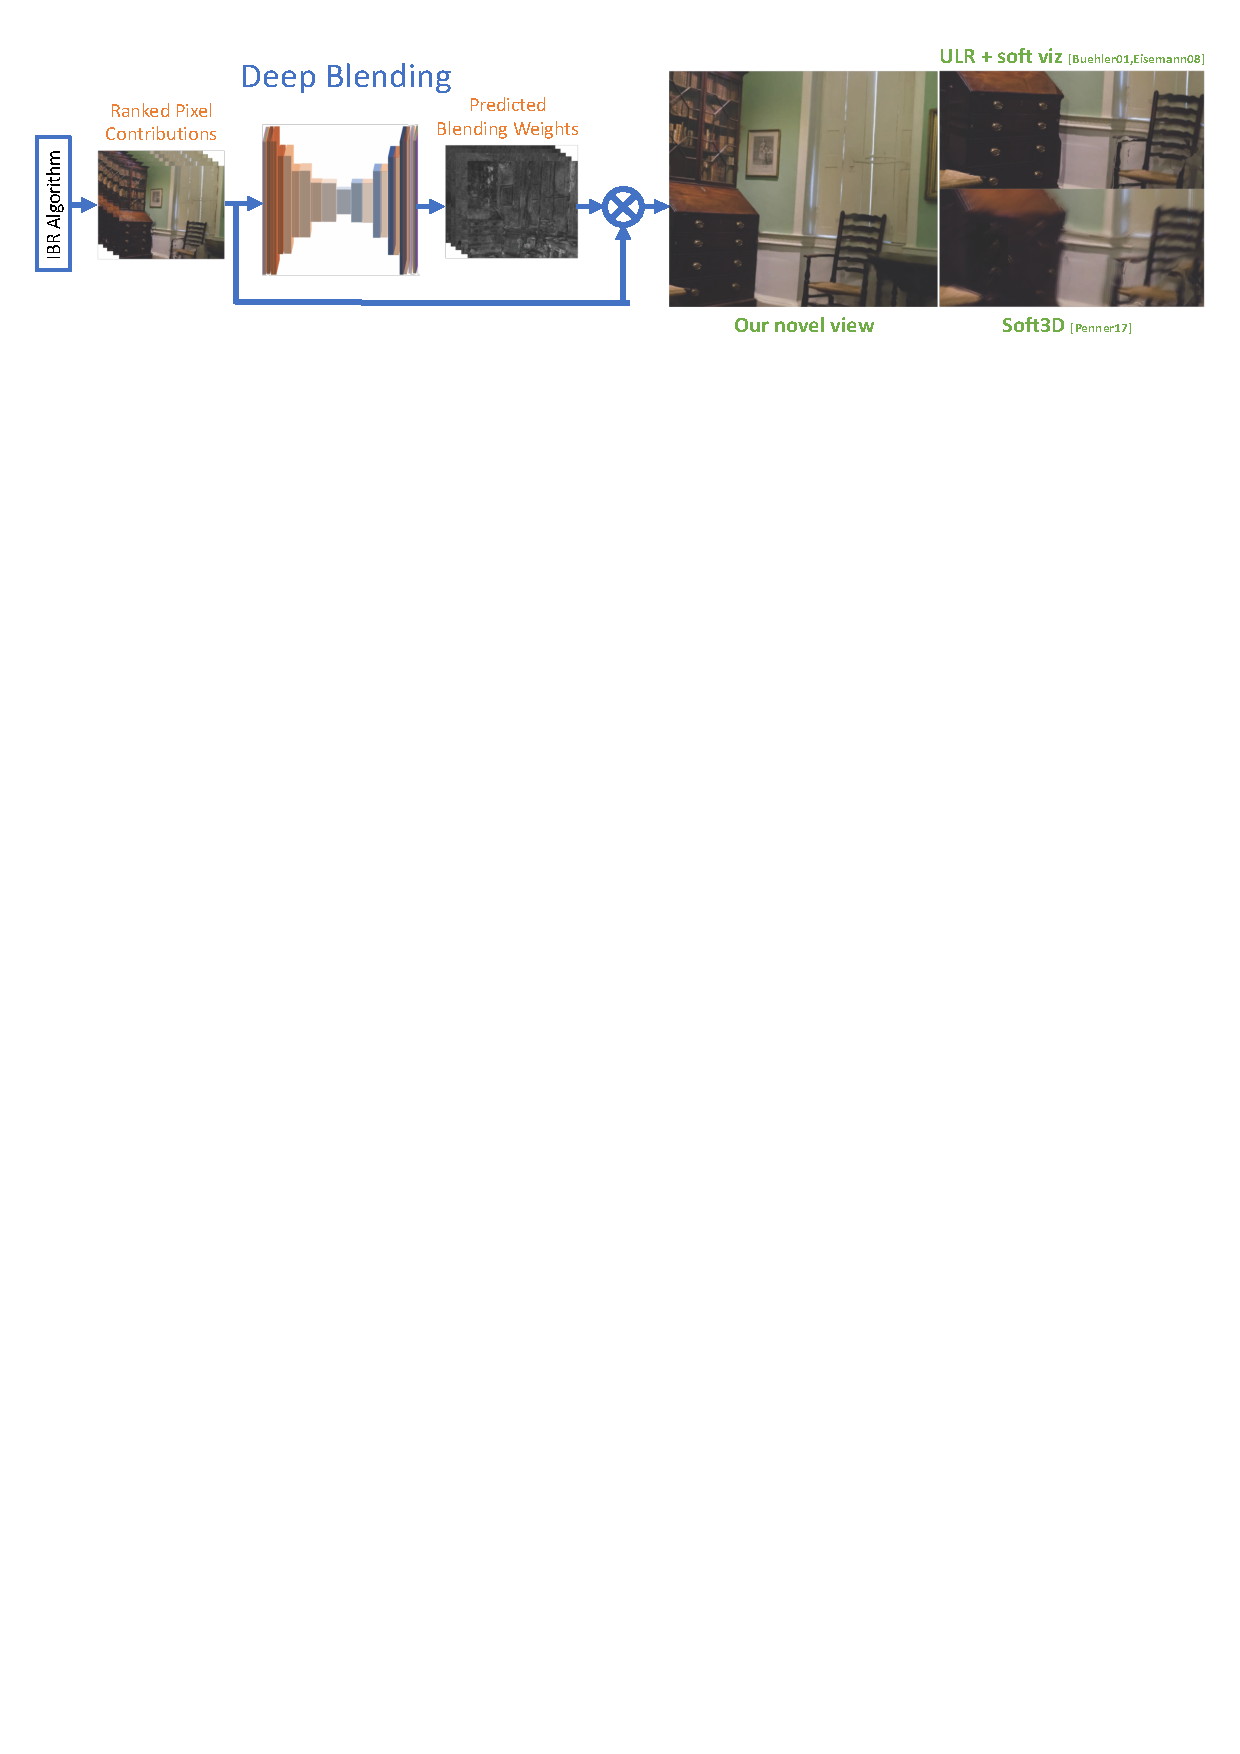
\includegraphics[width=0.95\textwidth]{figures/deepblending.pdf}
    \caption{DeepBlending\cite{hedman2018deep} 的框架结构,渲染效果较其他方法减少了伪影。}
    \label{fig:deepblending}
\end{figure}

为了解决上述问题,将经典的基于图像渲染的方法与现如今最火的深度学习网络的结合成基于 IBR 的神经渲染方法,这极大地提升了 IBR 的渲染效果。DeepBlending\cite{hedman2018deep}提出了一种广义网络来预测投影源图像的混合权重,以便在目标图像空间进行合成。DeepBlending 在室内场景中显示了惊人的效果,比经典的 IBR 方法具有更少的混合伪影,具体见图~\ref{fig:deepblending}。事实上,DeepBlending 是将 COLMAP\cite{schonberger2016structure} 和商用软件 Reality Capture 进行了结合,以此获取更为精细的几何结构信息。COLMAP 基于块匹配的多视图几何算法进行稠密重建,这能够非常好地重建场景中的细节,但是与此同时在纹理信息缺失的地方也会出现空洞。Reality Capture 的结果相对完整,但是对于场景级别的区域重建的较差。因此,上述两种方法是互补的,将它们进行结合可以获得非较为准确的几何模型信息,DeepBlending 就是使用上述几何信息,借助神经网络来学习如何将不一致的观测图像信息进行混合,最终确实获得了非常惊艳的效果。但是,该方法过于依赖 COLMAP 三维重建出的几何信息,当几何信息较少时渲染质量会严重下降并伴随伪影。此外,精细的三维重建会带来非常大的计算开销,这在实际中难以使用。因此这种经典的基于 IBR 的方法无法满足本系统的速度和质量需求。

%其他方法如 NPBG\cite{aliev2019neural} 和 NPCR\cite{dai2020neural} 使用比 mesh 更容易获得的点云作为三维代理几何体。由于点云自身的稀疏性特征,很可能会出现不应该观测到的点出现在新视角下,这是著名的 bleeding 现象。为了解决 bleeding 现象问题,NPBG 使用多分辨率的方式,将不同分辨率的特征图输入到后端网络中。不过,多分辨率的策略虽然解决了 bleeding 的问题,但是得到了相对模糊的渲染结果。	

\subsection{基于 NeRF 的新视图合成研究现状}
类似 DeepSDF\cite{park2019deepsdf},NeRF\cite{mildenhall2020nerf}借助深度学习的隐式表达方法,将三维几何场景中的光照和几何信息隐式表达在神经网络参数中,最后利用立体渲染的方法进行渲染。NeRF 算是基于图像的神经渲染方法中最具代表的工作了。NeRF 本身不需要任何的显式的几何信息,仅使用真实场景的 RGB 图像作为监督信号,使用深度神经网络自动推理相关几何以及光照信息。NeRF 凭借着其网络简单,渲染效果惊艳的特性,备受学术界和工业界的关注。自从 NeRF 的出现,基于神经辐射场的新视图合成相关工作开始大量涌现。

NeRF++\cite{zhang2020nerf++} 首次指出 NeRF 具有形状光线的歧义性问题,即 NeRF 在一个场景下训练好的网络,其对应的空间表示可能是错的,但是仍能在训练集上渲染出正确的结果。

%\begin{figure}[tbhp]
%    \centering
%    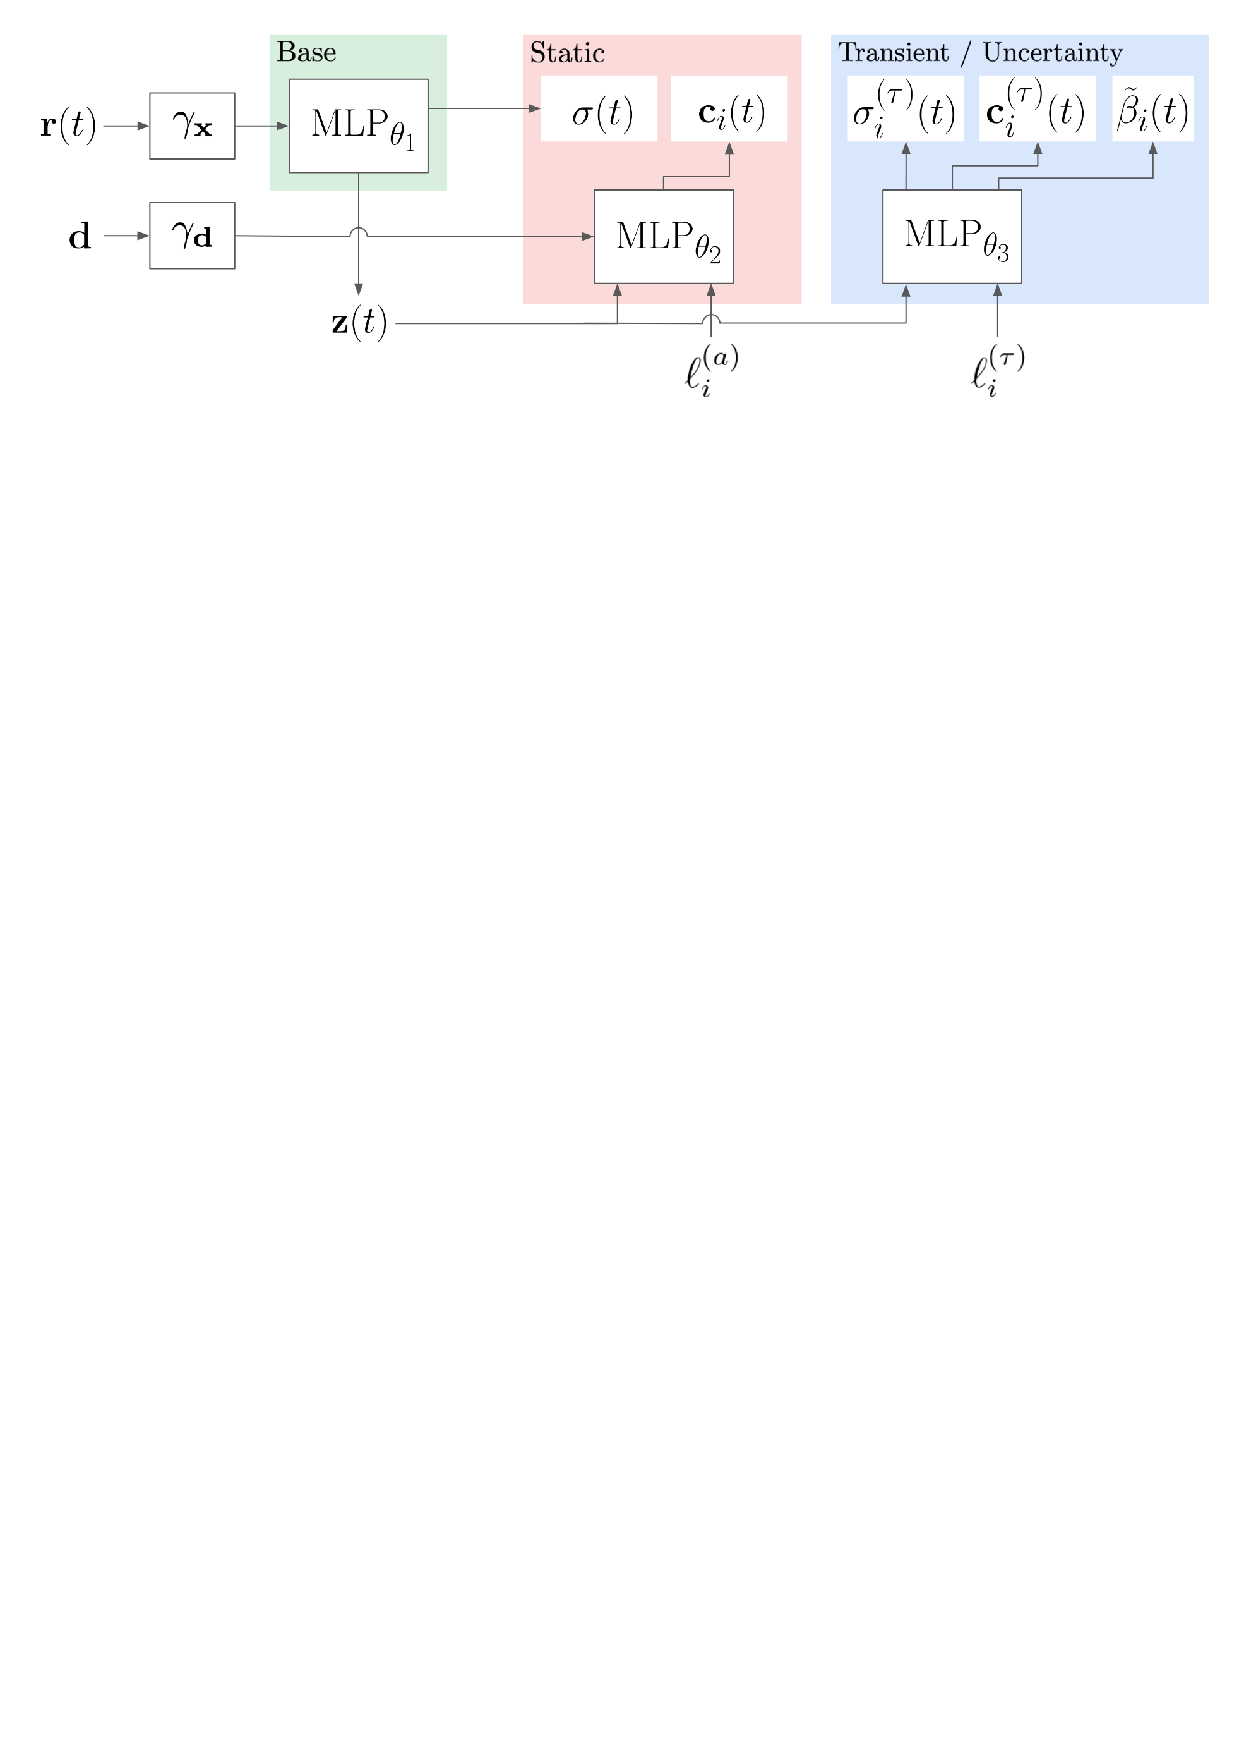
\includegraphics[width=0.95\textwidth]{figures/NeRF-W.pdf}
%    \caption{NeRF-W\cite{martin2020nerf}的网络框架示意图}
%    \label{fig:nerf-w}
%\end{figure}
%
%之后 NeRF-W\cite{martin2020nerf} (NeRF in the Wild) 对 NeRF 进行了另一种补充改进。由于 NeRF 假设输入的图像是由静态场景生成的图像,每张图所表示的场景具有相同的光照条件和几何结构,这在实际中是很难保证的。对于这个问题,如图~\ref{fig:nerf-w}所示,NeRF-W 给每张图片都预先编码了两个固定向量,分别是 $l_i^{\left(a\right)}, l_i^{\left(\tau\right)}$。其中,$l_i^{\left(a\right)}$ 是用来学习当前的光照条件,而 $l_i^{\left(\tau\right)}$ 是用来学习当前图像是否有动态物体遮挡,将这两个embedding 输入网络会输出一个不确定度。以上的做法让 NeRF-W 在真实场景下能够表现地更加鲁棒,在光照条件变化以及动态的场景下都取得了非常好的效果。

Yen-Chen等人\cite{yen2020inerf}基于位姿估计方法给 NeRF 提供了新的改进思路,推出了新工作 iNeRF。NeRF 在处理真是数据集的时候,位姿是通过COLMAP\cite{schonberger2016structure}进行计算的,然而这并不能获得绝对精准的位姿,也即送入网络的采样点是不准确的,那么也无法准确拟合真是场景的神经辐射场。如图~\ref{fig:inerf} 所示的是 iNeRF 的网络框架,注意到,颜色的均方误差对坐标是可微的,而坐标对相机位姿也是可微的,因此,可以在训练神经辐射场的同时对位姿进行优化,具体是采用神经网络的反向传播算法进行优化的。此外,为了更有效地优化位姿,iNeRF 使用了 ROI 采样方式,即对感兴趣的区域进行采样优化,这样能显著缓解直接采样一张图片带来的内存开销大的问题。iNeRF 通过位姿矫正,最终在真实场景下显著提升了 NeRF 的渲染质量。不过,由于训练时每一张图都要单独优化位姿,而渲染时相机位姿仍然是不准确的,因此本系统暂不考虑位姿的问题。

\begin{figure}[tbhp]
    \centering
    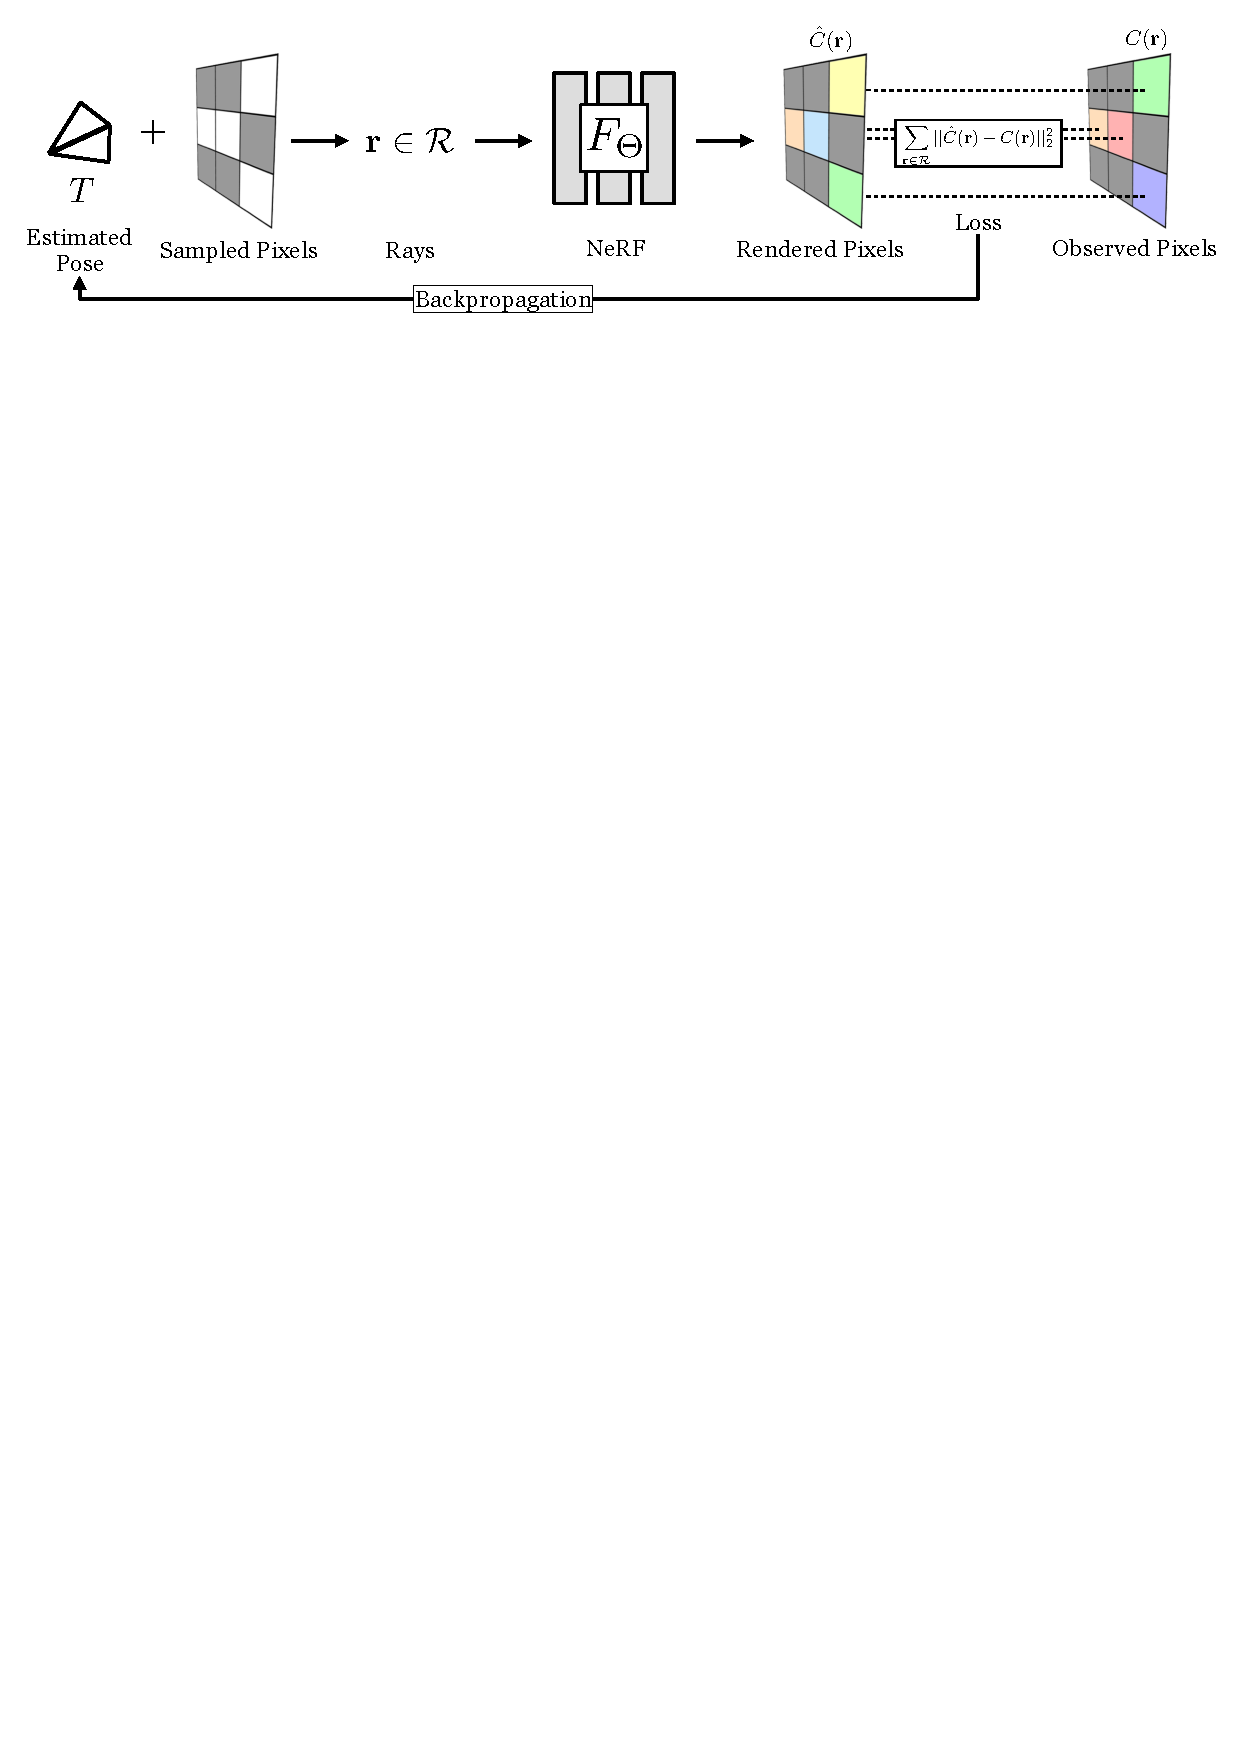
\includegraphics[width=0.95\textwidth]{figures/iNeRF.pdf}
    \caption{iNeRF\cite{yen2020inerf}的网络框架示意图}
    \label{fig:inerf}
\end{figure}

上述方法都还是基于多层感知机 (MLP, Multilayer Perceptron) 训练的。下面介绍一些对 NeRF 网络上进行的一些改进的工作。PixelNeRF\cite{yu2020pixelnerf} 使用卷积神经网络 (Convolutional Neural Networks, CNN) 提取的特征,仅需要少量图片作为输入就可以合成新视角下的图像,并有一定的泛化能力。GRF\cite{trevithick2020grf}使用 CNN 提取包含光线属性的特征,并使用 attention 机制将采样点在不同视角下的特征进行聚合,极大地提升了渲染质量。GRAF\cite{schwarz2020graf} 使用对抗生成网络 (Generative Adversarial Networks, GAN) 对 NeRF 进行改进,使之具有较强的泛化能力。但是,以上这些基于网络的改进方法都使得网络变得过于复杂,有些违背 NeRF 网络简洁的初衷,会使得训练和渲染的时间过长,这不能满足用户对于快速合成新视图的需求,几乎无法应用到实际的系统中。

\begin{figure}[htb]
	\centering
	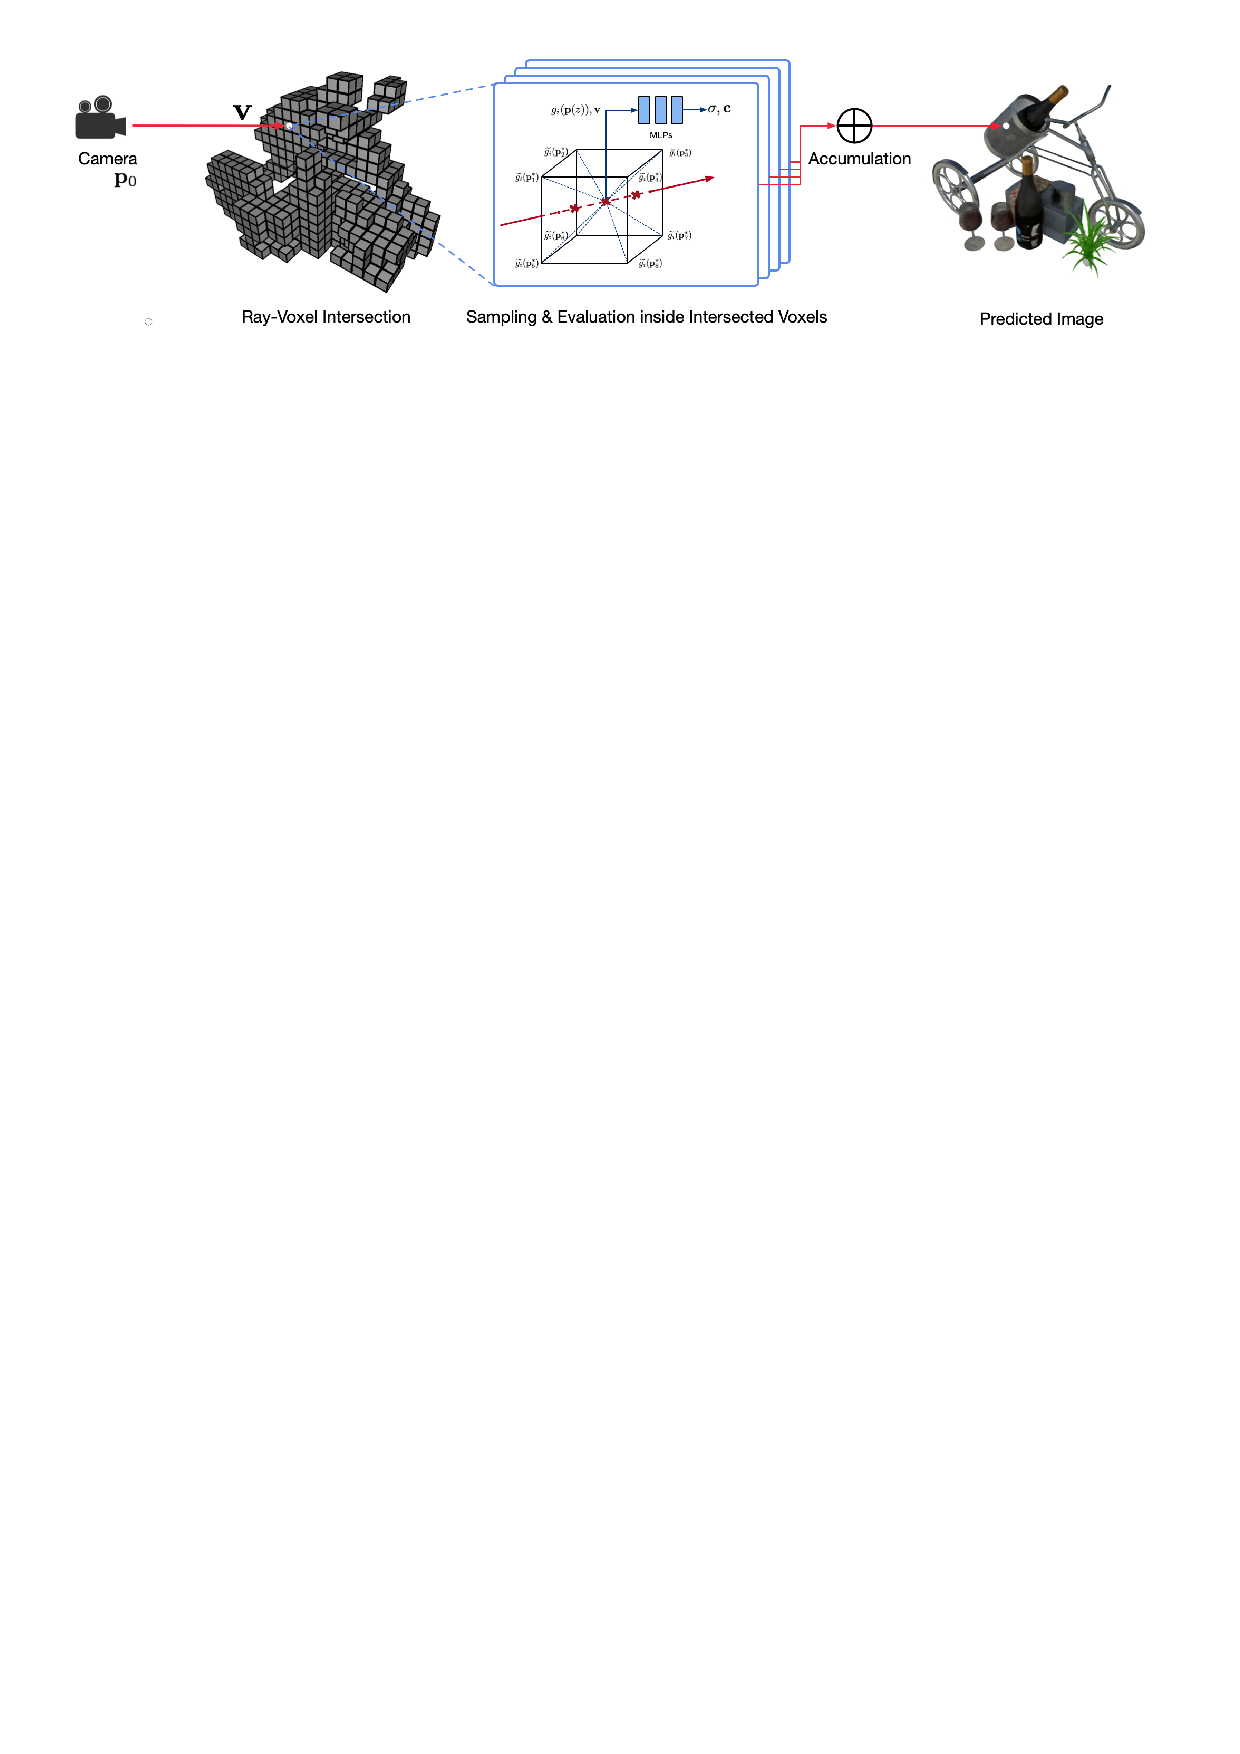
\includegraphics[width=0.95\textwidth]{figures/NSVF.pdf}
	\caption{NSVF\cite{liu2020neural}的网络框架示意图}
	\label{fig:nsvf}
\end{figure}

下面介绍一些基于 NeRF 的加速方法。由于 NeRF 需要在相机光线上进行大量的采样,这些采样点都要经过网络,而 NeRF 自身又使用了两个网络进行训练,因此 NeRF 的渲染是很慢的。如图~\ref{fig:nsvf},为了给 NeRF 加速,NSVF\cite{liu2020neural} 首先提出将空间划分为若干体素,使用自我裁剪的方法去掉体密度较小的体素,渲染的时候只需找到相机光线第一个穿过的体素,根据该体素八个顶点对应的特征进行插值编码并送入下游 MLP 预测出颜色和体密度,这避免了大量的采样计算,显著加速了新视图合成的过程。但是,NSVF 仅适用于简单的三维物体,在复杂的真实场景下渲染新视图的质量较差,甚至会出现鬼影,因此并不适合在本系统上使用。Lindell等人\cite{lindell2020autoint}提出了一种利用自动积分来进行渲染加速的方法 AutoInt。AutoInt 是通过隐式网络学习到闭式解求积分,从而取代了 NeRF 的数值积分,最终能为 NeRF 渲染过程加速10倍。不过,就 PSNR 来看,AutoInt 在合成数据集 Synthetic-NeRF 上平均比 NeRF 低\SI{5.4}{dB},这是一种重视加速但牺牲了很多质量的方法,并没有真正做到在不失精度的情况下对渲染进行加速。上述介绍的加速方法未能保证不损失精度情况下对 NeRF 进行加速,不符合本系统的需求,因此本文最终依旧使用最经典应用场景最丰富的 NeRF 技术并对其进行无精度损失的加速,最终完成整个快速新视图合成系统的构建。

\section{本文的主要工作与贡献}
% 基于神经辐射场的快速新视图合成系统的设计与实现中存在以下一些问题:1) 当前市场上的三维渲染的软件难以根据稀疏视图,在任意视角下渲染出高质量的新视图;
% 2) 目前的三维渲染系统大都需要根据深度信息进行三维建模,这需要使用 RGBD 相机,对硬件设备要求较高;
% 3) 目前市场上还没有直接可应用的面向快速新视图合成的交互系统;4) 现有的新视图合成模型需要在空间内进行大量采样,计算时间成本较高,难以完成 PC 端的交互需求。

本文将 NeRF 技术和查询表技术进行有机融合,设计并实现了基于神经辐射场的快速新视图合成系统。本文根据 NeRF 的特性提出了基于神经辐射场进行加速合成新视图的框架, 将其命名为 F-NeRF,通过 NeRF 预测的体密度有效地提取到物体的几何结构并缓存到查询表中,这一方面辅助了获取物体表面附近的对计算颜色有高贡献的采样点,另一方面减少了一个网络的开销,同时也简化了网络,这显著加速了渲染的过程。最后,本文将这 F-NeRF 这一方法有效地部署到 PC 端,将其实现成可交互的系统。

具体地,本文的主要工作与贡献如下:
\begin{enumerate}
    \item [1)] 本文基于 NeRF 预训练的网络预测的体密度信息构建出一个可以表征在物体内外的查询表结构,这一方面直接减少了查询表的尺寸,另一方面该查询表可以直接为空间内任意一点提供 NeRF 网络中间层的特征,这加快了神经网络的正向传播速度。
    \item [2)] 在缓存了上述查询表的基础上,本文改进了 NeRF 的采样过程,通过查询表找到光线上离物体表面最近的内点,使得 NeRF 可以仅在此点附近进行采样,从而不必再使用两个网络,这显著加速了 NeRF,同时这正是本文的核心贡献。
    \item [3)] 为了补偿查询表分辨率不够带来的精度损失,本文对 F-NeRF 进行再训练,将渲染质量提升到原 NeRF 的水平。
    \item [4)] 本文在公开的数据集上做了大量对比验证实验。在公开合成数据集 Synthetic-NeRF 和真实场景数据集 LLFF-NeRF 上,与 NeRF 相比,我们提出的 F-NeRF 方法分别加速 3.2 倍和 3.4倍。 
    \item [5)] 本文设计并实现了基于 NeRF 的快速新视图合成的系统,完成了相应的 PC 端的应用,并对该系统进行了详细的需求分析以及架构设计,最后将本文的方法实现并部署到了 PC 端,经过详细地测试,该系统满足实际应用需求。
\end{enumerate}

%1) 使用预训练的 NeRF 网络,构建出一个可以表征在物体内外的查询表,该查询表可以直接为空间内任意一点提供 NeRF 网络中间层的特征,这加快了神经网络的正向传播速度。
%2) 在缓存了上述查询表的基础上,本文改进了 NeRF 的采样过程,通过查询表找到光线上离物体表面最近的内点,使得 NeRF 可以仅在此点附近进行采样,从而不必再使用两个网络,这显著加速了 NeRF,同时这正是本文的核心贡献。3) 本文设计并实现了基于 NeRF 的快速新视图合成的系统,完成了相应的 PC 端的应用,并对该系统进行了详细的需求分析以及架构设计,最后将本文的方法实现并部署到了 PC 端,经过详细地测试,本文方法在合成场景和真实场景下的渲染速度对 NeRF 分别加速3.2倍和3.4倍,该系统满足实际应用需求。


\section{本文的章节安排}

第一章是绪论,主要阐述了本文研究工作的背景与意义,指出了本文研究问题的难点,并介绍了本文的主要研究工作和贡献,对国内外相关工作的研究现状的充分调研与分析,最后对本文的组织架构进行安排。

第二章是相关理论和技术,主要介绍了基于神经辐射场的快速新视图合成系统应用的核心技术和算法。

第三章是本文的主要工作,主要介绍了本文方法的问题定义,本文方法的预备工作,然后详述了我们改进的基于神经辐射场的新视图合成加速方法。

第四章是本文的实验部分。主要阐述了实验的基本设置,包含开发环境、数据集等等,其次介绍了实验实现的具体细节以及相关评测指标。最后通过大量对比实验来验证本文提出的方法的有效性,同时对一些实验结果进行分析和讨论。

第五章是系统设计与实现,主要介绍了将本文提出的 F-NeRF 方法应用到系统上的具体实现与架构设计。详细阐述了本系统的需求分析,包含主要用例分析,以及具体的系统架构设计,最后介绍了将本系统的模型移植到 C++ 代码上的方法。

第六章是系统的部署与展示,主要介绍了本文系统的开发与运行环境,对经典的测试用例进行了详尽的步骤说明,根据用例步骤完成了功能测试。从测试结果看,系统各项功能均能正常运行,合成新视图速度快且质量高。

第七章为总结和展望部分。总结了本文的主要工作和贡献,并指出工作中的不足之处。提出在未来研究过程中的可能的研究方向,并对可继续完善的方面进行展望。
% \begin{enumerate}
%     \item 主体部分包括引言 (前言),国内外文献综述,正文, 结语,参考文献。要求图表清晰,叙述流畅,章节有序,层次 分明。\\
%     引言 (前言)部分内容主要为本研究课题的学术背景及理论与实际意义;本研究课题的来源及主要研究内容;建立研究的线索与思路。

%     \item 文中的图、表、公式等,一律用阿拉伯数字按章顺序编号。如图 1-1、图2-2, 表 1-1、表 2-1,公式 (1-1) 等。图序及图名置于图的下方,居中排列;表序及表名置于表的上方,居中排列。详见第\ref{figures_tables}章的说明。

%     \item 参考文献
%     \begin{enumerate}
%         \item 参考文献为论文中所有引文、引用观点以及对论文有重要影响和启发的文献;
%         \item 参考文献按在论文中出现的先后依次排序;个别学科若通用该学科惯用的排序规范,可以例外;
%         \item 参考文献内容一般排列在论文末尾 (论文篇幅较大且引用文献较多的,可在每章末尾注出),序码与论文加注处对应;
%         \item 参考文献标注格式: 使用国标GB/T 7714-2015标准, 建议使用工具自动控制引文格式, 
%         以保证格式规范。
%         该\LaTeX{}模板已经对引文格式做了配置,
%         用户需要将所需参考文献的信息存在 \texttt{bib} 格式的文件\texttt{ref/refs.bib}中, 
%         通过 \verb|\cite{}|命令在恰当位置引用 (详见第\ref{citations}章的说明)。
%         \texttt{bib}文件可从文献管理工具导出或自己用 \texttt{JabRef} 等软件编辑。
%     \end{enumerate}

%     \item 注释:可以用 “脚注”或 “文后注”来标注引用著作中的一些观点和案例,但全文标注方式应统一。
% \end{enumerate}


%     \cleardoublepage
%     % !TeX root = ../main.tex

\chapter{相关技术和理论概述}\label{equations}
本文主要研究的内容是神经辐射场在新视图合成上的加速,因此本章首先主要介绍神经三维形状表示法,新视图合成和基于图像的渲染方法。随着深度学习的发展,当今效果最佳的新视图合成算法都是基于深度学习的,因此接下来会概述深度学习的原理和发展状况,并重要介绍基于深度学习的神经辐射场的立体渲染方法。最后介绍一下查询表的概念,以及查询表在逐点网络上的加速应用,为本文方法的展开做好铺垫。

\section{神经三维形状表示法}
三维物体的形状表示有多种方法,传统的基于数据驱动的三维学习表示方法可以总体上分为三类:基于点,基于网格,基于体素的方法。此外,还有最新的基于深度学习的三维形状表示方法,下面对以上四种表示方法分别进行阐述。

\subsection{基于点的表示方法} 
基于点的方法一般指的是点云(如~\ref{fig:stanfordRabbit}所示的第一个)这种表示,点云是指空间中一组点的集合,每一个点都包含 X,Y,Z 三个坐标。它是一种轻量级的三维表示方式,与匹配许多传感器(例如雷达,深度相机)提供的原始数据非常匹配,因此非常适合应用在三维学习技术上。例如 PointNet\cite{qi2017pointnet,qi2017pointnet++} 这篇非常经典的点云工作,使用最大池化操作来提取全局特征,之后这项技术被广泛用作点生成网络\cite{yang2017foldingnet,achlioptas2018learning}的编码器。此后点云学习方面又涌入了大量的 PointNet 风格的相关工作。然而,点云这种表示方法有着很明确的限制,它们不适用于描述拓扑结构,同时也不适合用以生成紧致的表面。

\subsection{基于网格的表示方法}
许多方法使用预定义模板的网格,它们表征了一系列相似形状的物体,例如可变形的人体部位,其中一些模型\cite{2017Deformable}展示了高保真的形状生成结果。其他的最近工作\cite{baque2018geodesic}使用多边形立方体映射\cite{tarini2004polycube}对形状进行优化。虽然模板网格的使用很方便,并且自然地提供了三维对应,但它只能对具有固定网格拓扑的形状进行建模。其他基于网格的方法使用已有的\cite{sinha2016deep,maron2017convolutional}或者学习的\cite{groueix2018papier,ben2018multi}参数化技术通过二维平面来描述三维曲面。这种表示的质量取决于参数化算法,这些算法通常对输入网格质量和切割策略非常敏感。为了解决这个问题,最近的数据驱动方法\cite{yang2017foldingnet}学习深度网络的参数化任务。然而,他们报告说需要多个平面来描述复杂的拓扑,但是生成的曲面片没有缝合,即生成的形状没有闭合。为了生成闭合网格,可以使用球体参数化\cite{groueix2018papier,ben2018multi},但生成的形状仅限于拓扑球体。其他与网格学习相关的工作建议对网格\cite{defferrard2016convolutional,verma2018feastnet}或一般图\cite{bruna2013spectral}使用新的卷积和池化运算。网格表示三维物体的直观感受如~\ref{fig:stanfordRabbit}所示。

\subsection{基于体素的表示方法}
在三维计算机图形学上,体素代表了三维空间中规则格点所对应的值。与二维位图中的像素一样,体素本身通常不使用其值显式编码其位置(即坐标)。取而代之的是,渲染系统根据其相对于其他体素的位置(即其在构成单个体积图像的数据结构中的位置)来推断体素的位置。体素算是像素由二维空间直接推广到三维空间,有着不少共性。基于体素的学习方法中最直接的变体就是占据栅格。但是由于计算和内存开销呈三次方的增长趋势,因此当前的方法只能处理较低分辨率的情况。因此,基于体素的方法\cite{20153D,Choy20163D}无法保留精细的形状细节,由如~\ref{fig:stanfordRabbit}所示的第三个图就能明确这一点,此外,体素在视觉上显示与高保真度形状有显著差异,因为渲染时法线不平滑。基于八叉树\cite{Tatarchenko2017Octree,riegler2017octnet,hane2017hierarchical}的方法一定程度上减轻了稠密体素方法的计算和内存限制,但是提升后的分辨率依然没有产生很好的视觉响应。

\begin{figure}[t]
  \centering
  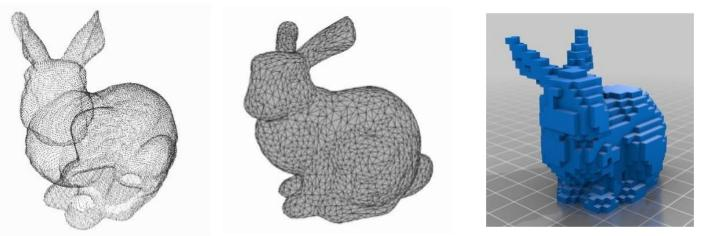
\includegraphics[width=0.9\linewidth]{stanfordRabbit.jpg}
  \caption{三种传统的三维表示方式(点云,网格,体素)}
  \label{fig:stanfordRabbit}
\end{figure}

\subsection{基于深度学习的表示方法}
计算机视觉中最近一个有前景的方向是用多层感知机 MLP 的权值编码对象和场景,MLP 直接从三维空间位置映射到形状的隐式表示,例如该位置的有符号距离\cite{curless1996volumetric},如图~\ref{fig:sdf}所示是有符号距离函数 (Signed Distance Fuction, SDF)在三维表示上的应用。然而,这些方法到目前为止还无法再现具有复杂几何体的真实场景,其保真度与使用离散表示(如三角形网格或体素网格)表示场景的技术相同。

最近的工作通过优化将 xyz 坐标映射到 SDF 函数\cite{jiang2020local,park2019deepsdf,chabra2020deep}或占据域\cite{genova2020local,mescheder2019occupancy}的深度网络,研究了连续三维形状作为水平集的这种隐式表示。然而,这些模型受到三维几何体 ground truth 的需求的限制,这些几何体通常是从合成的三维形状数据集(例如如 ShapeNet\cite{chang2015shapenet} )获得的。随后的工作通过构造可微的渲染函数,使得神经隐式形状表示仅使用 2D 图像进行优化,从而放宽了对三维形状 ground truth 的要求。Niemeyer 等人\cite{niemeyer2020differentiable}将曲面表示为 3D 占据场,并使用数值方法找到每条光线的曲面交点,然后使用隐式微分计算精确导数。每个光线相交位置都作为神经 3D 纹理场的输入,该纹理场预测该点的颜色。Sitzmann 等人\cite{sitzmann2019scene}使用了一种不太直接的神经 3D 表示法,只需在每个连续的 3D 坐标上输出一个特征向量和 RGB 颜色,并提出了一种可微绘制函数,该函数由一个沿每条射线行进的递归神经网络组成,以确定曲面的位置。

\begin{figure}[t]
  \centering
  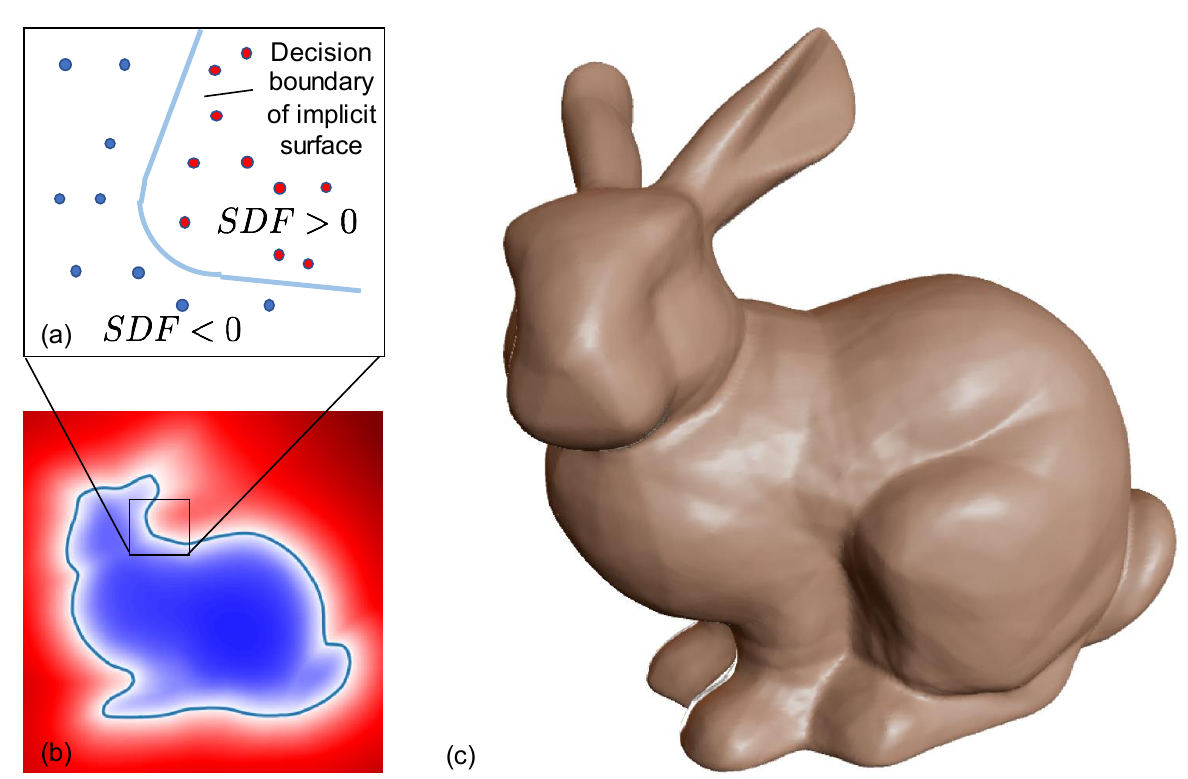
\includegraphics[width=0.8\linewidth]{sdf.png}
  \caption{SDF 函数表示法应用于斯坦福兔子,图片来自于 DeepSDF\cite{park2019deepsdf}}
  \label{fig:sdf}
\end{figure}

\section{新视图合成和基于图像的渲染}
新视图合成在计算机视觉与计算机图形学这样的交叉领域上是一个长期的问题。所谓新视图合成指的是给定一系列(或者单张)已知相机位姿的视图,由这些视图合成出未知位姿的视图。新视图合成的过程如图~\ref{fig:novelviewsynthesis}所示。对于给定稀疏视角采样的新视角合成问题,计算机视觉和图形学社区在从观测到的图像中预测传统几何表示的问题上取得了很多进展。一类流行的方法是使用具有要么漫反射\cite{Waechter2014Let}的,要么依赖视角\cite{debevec1996modeling, wood2000surface}的外观的那些 mesh-based(基于网格) 的场景表示。可微分的光栅化器\cite{loper2014opendr,chen2019learning,genova2018unsupervised,liu2019soft}或路径跟踪器\cite{li2018differentiable,nimier2019mitsuba}可以直接通过使用梯度下降法来优化再现一组输入图像的网格表示。然而,基于图像重投影的网格梯度下降的优化是十分困难的,可能是由于局部极小值或 loss 的调整不佳所致。此外,这种策略\cite{li2018differentiable}要求在优化之前提供具有固定拓扑的模板网格作为初始化,这通常对于不受约束的真实场景是不可用的。

另一类方法使用体积表示法来解决从一组输入 RGB 图像中进行高质量逼真的视图合成的任务。体积表示法是能够真实地表达复杂的形状和物体,非常适合基于梯度的优化,比基于网格的方法产生的视觉干扰更少。早期的体积方法\cite{kutulakos2000theory,szeliski1998stereo}使用观察到的图像直接为体素网格着色。最近,几种方法\cite{flynn2019deepview,mildenhall2019local,srinivasan2019pushing,zhou2018stereo}使用了多个场景的大型数据集来训练深层网络,这些深层网络从一组输入图像中预测采样的体积表示,然后使用其中一种 alpha 合成\cite{porter1984compositing}或沿光线学习的合成,以在测试时渲染新视图。其他工作需要针对每个特定场景优化了卷积神经网络和采样体素网格的组合网络,这样 CNN 可以补偿来自低分辨率体素网格\cite{sitzmann2019deepvoxels}的离散化伪像或允许预测的体素网格根据输入时间或动画控制而变化。尽管这些体积化的技术在新视图合成中取得了令人印象深刻的效果,但是由于它们是离散采样的,它们在时间和空间上的复杂性从根本上限制了它们缩放到高分辨率图像的能力,渲染高分辨率的图像需要 3D 空间的更精细的采样。NeRF 通过在全连接的深度神经网络的参数范围内编码连续的体积来规避此问题,这不仅比以前的体积方法产生了更高质量的渲染,而且只需要这些采样体积表示的存储成本的一小部分。

\begin{figure}[t]
  \centering
  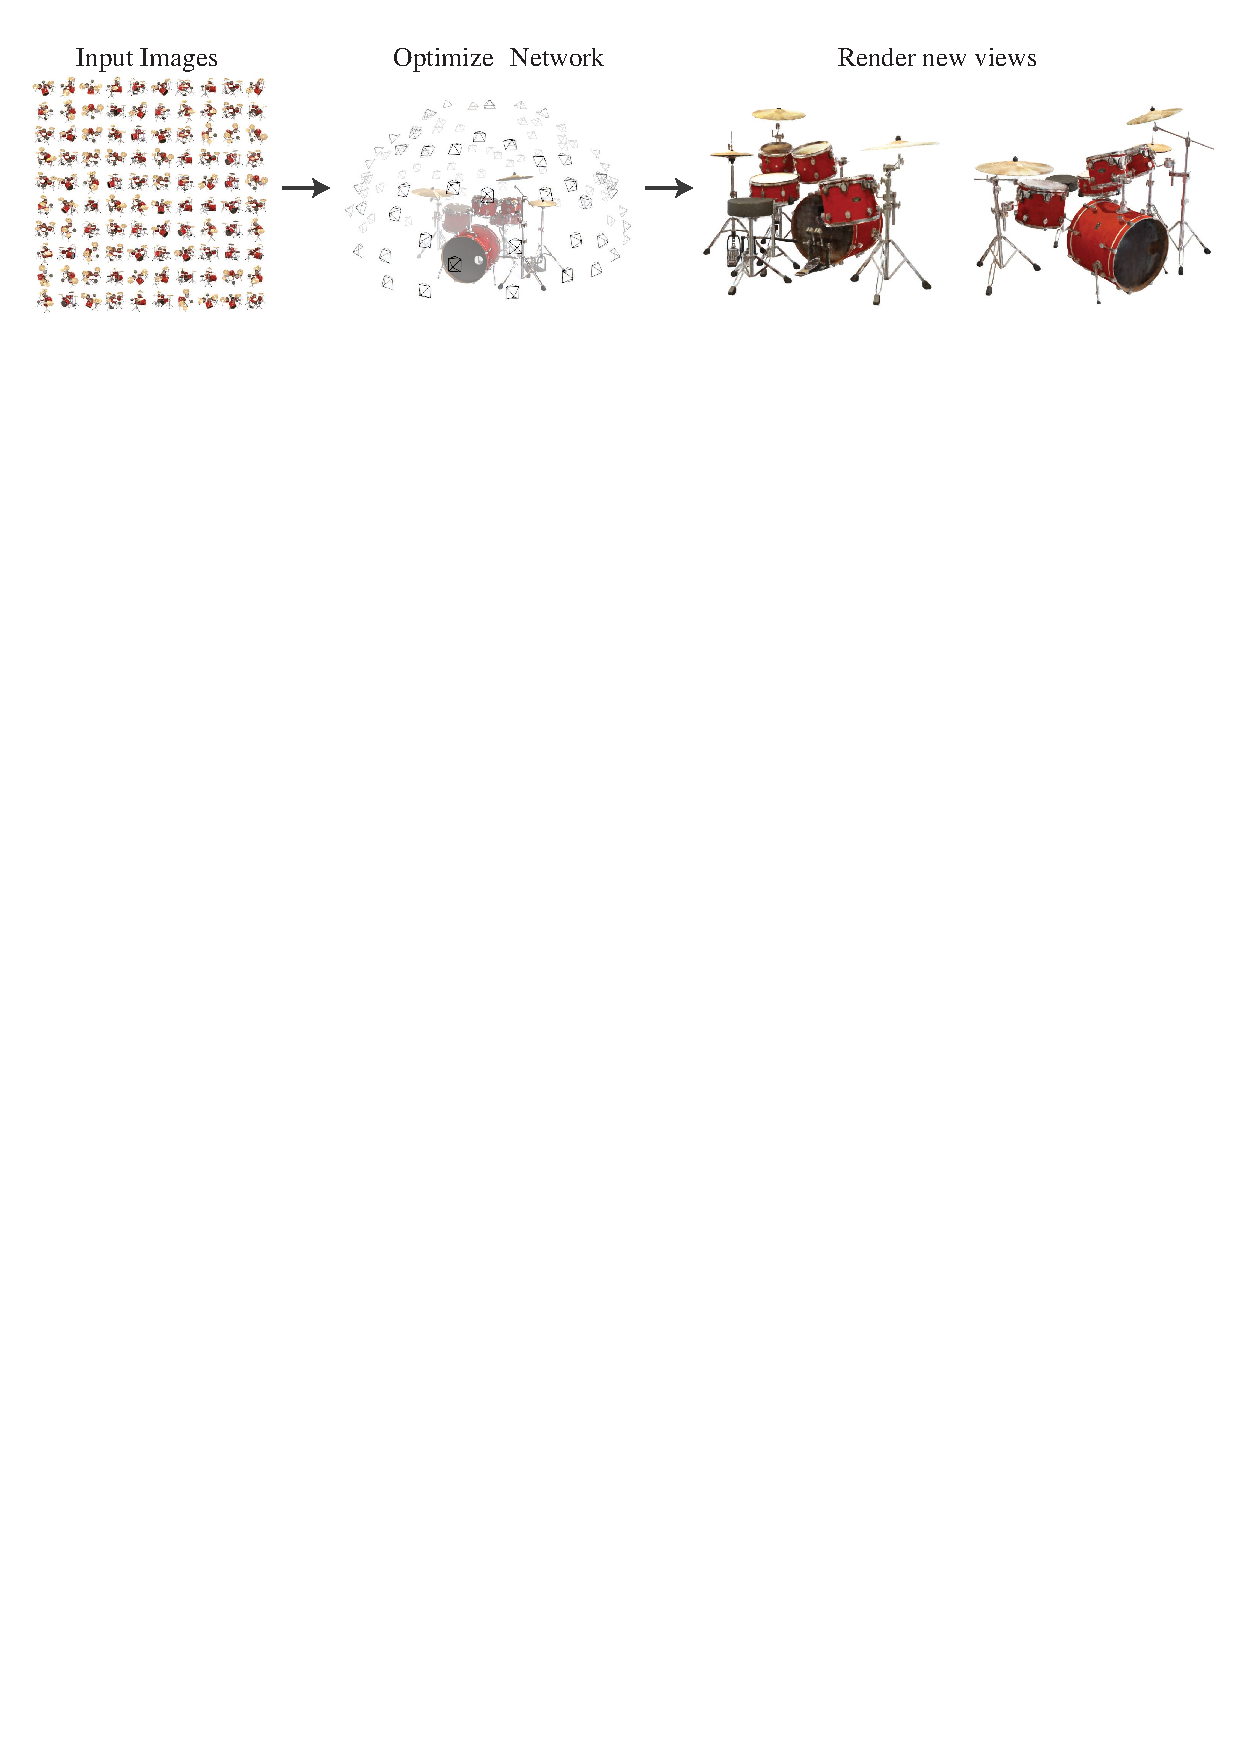
\includegraphics[width=0.95\linewidth]{figures/drums.pdf}
  \caption{新视角合成的过程\cite{mildenhall2020nerf}}
  \label{fig:novelviewsynthesis}
\end{figure}

\section{深度学习发展概述}
深度学习 (Deep Learning, DL) 是机器学习的一个分支,是一种以人工神经网络(如图~\ref{fig:neuralNetwork})为架构进行表征学习的方式。深度学习有着非常悠久的历史,最早可以追溯到20世纪40年代\cite{goodfellow2016deep}。学习可以是有监督的、无监督的,也可以是半监督的。

深度学习发展到现在,得益于 GPU 性能的巨大提升,已有诸如深度神经网络 (Deep Neural Network, DNN) ,深度置信网络\cite{hinton2009deep} (Deep Brief Network, DBN) ,循环神经网络\cite{rumelhart1986learning} (Recurrent Neural Network,RNN) ,卷积神经网络\cite{lecun1995convolutional} (Convolutional Neural Networks, CNN) 等深度学习框架被应用于计算机视觉、语音识别、自然语言处理、音频识别和生物信息学上。

由于本文主要涉及计算机视觉和计算机图形学的知识,因此接下来两小节会介绍这些领域最常用的两个网络架构,卷积神经网络和残差网络 Resnet 。

\begin{figure}[t]
  \centering
  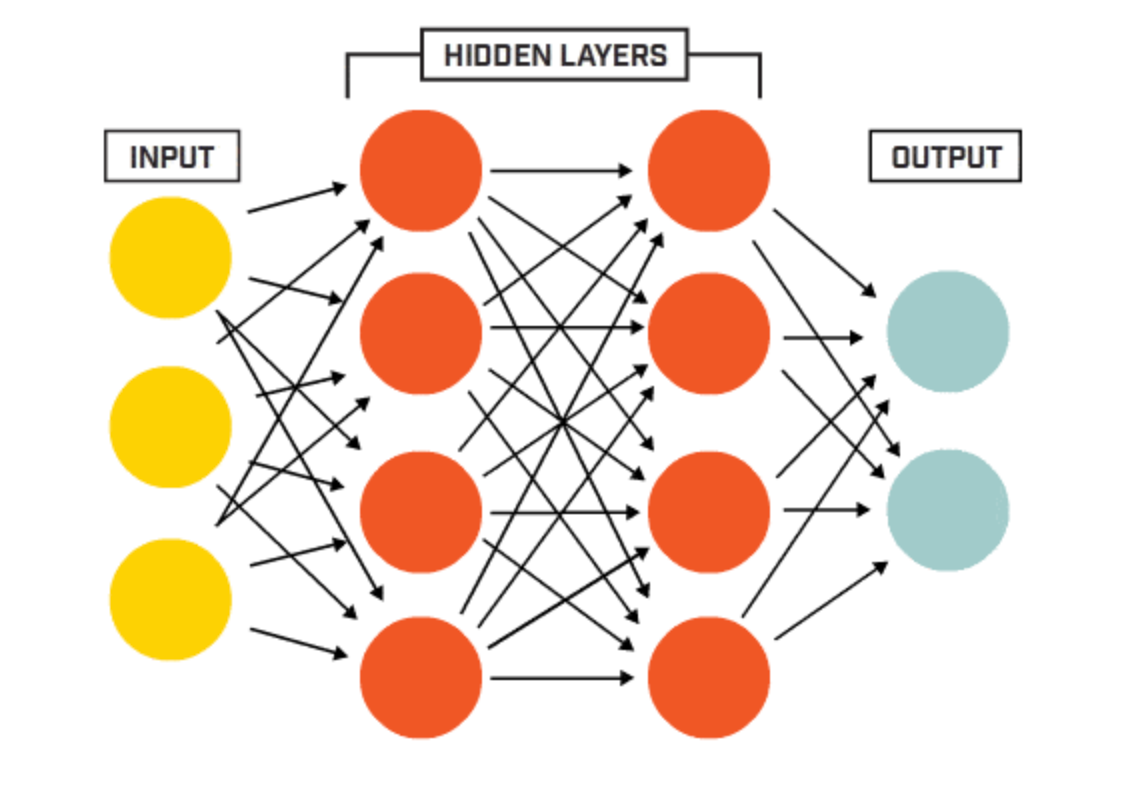
\includegraphics[width=0.9\linewidth]{figures/fc.png}
  \caption{神经网络示意图}
  \label{fig:neuralNetwork}
\end{figure}

\subsection{卷积神经网络}
要具体阐述卷积神经网络,就不得不先提到 MLP ,如图~\ref{fig:neuralNetwork},主要由输入层,隐藏层和输出层三个模块。除了输入层和输出层,隐藏层经常采用 sigmoid 和 tanh 作为激活函数,这里激活函数的作用是为了增加网络非线性拟合能力,若是没有激活函数,即使是使用多层网络进行训练,实际上只相当于一层,只能进行线性拟合,没有很大的作用。不过上述两种激活函数在输入太小或者太大的时候会造成梯度接近于0,这使得梯度更新十分缓慢甚至可能消失,网络从而无法训练下去。与 tanh 相比,sigmoid 还有个非常不利于学习的问题,那就是 sigmoid 函数的值域是$[0,1]$,也因此输出的均值不会为0,这非常不利于下一层的学习。为了解决上述问题,Glorot 等人\cite{glorot2011deep}提出了 ReLU 函数,解决了在输入为正数时梯度消失的问题,此外由于计算比 sigmoid 和 tanh 简单,前向传播和反向传播也都相应更快。

对于正向传播,$l$层的输出和$l-1$层的关系始终可以由下列公式来表达,而与网络深度无关。
\begin{equation}
    a^{l} = \sigma(z^{l}) = \sigma(f(a^{l-1})),
\end{equation}
其中$z^l = f(a^{l-1})$,$f$表示第$l$层网络对应的映射函数,$a^{l-1}$表示前一层的输出(也是第$l$层的输入,$\sigma$表示激活函数)。而反向传播则可用链式法则来进行每一层的求导,计算出梯度。

但是对于图像这种数据来说,全连接网络有着很大的问题,一方面,比如即便是$256 \times 256 \times 3$这样的小图像也需要数十万的参数,这么多参数会使得网络的训练难以进行下去;另一方面,图像数据不像其他任务中的数据,图像本身具有一定的高级语义,为了更好处理地处理像图像这样的二维数据,卷积神经网络应运而生。CNN是一种前馈神经网络,由一个或多个卷积层和顶端的全连接层(对应经典的神经网络)组成,同时也包括共享参数和池化层。这一结构使得卷积神经网络能够利用输入数据的二维结构。这一模型也可以使用反向传播算法\cite{rumelhart1986learning}进行训练。相比较其他深度、前馈神经网络,卷积神经网络需要考量的参数更少,使之成为一种颇具吸引力的深度学习结构。

\begin{enumerate}
    \item 卷积层 \\
    卷积层的功能实际上是对输入进行特征提取。卷积层一般会包含多个神经元,或者叫做卷积核,组成卷积核的每一个元素都会包含一个权重和一个偏移量 (Bias Vector)。卷积核在工作的时候会有规则的扫过输入的特征,对卷积核大小范围内的特征做矩阵乘法并求和,最后再叠加上偏移量。
    
    对一张二维图像$X$,卷积层的输出可表示为
    \begin{equation}
        y_{ij} = \sum_{u=1}^{m}\sum_{v=1}^{n}w_{uv} * x_{i-u+1,j-v+1},
    \end{equation}
    其中$x$表示输入图像$X\in{R^{M\times N}}$的一个像素大小,$w$是卷积核$W \in R^{m\times n}$的参数,一般地$m << M$,$n << N$。
    二维卷积的示意图如图~\ref{fig:2dconv}
    \begin{figure}[htbp]
        \centering
        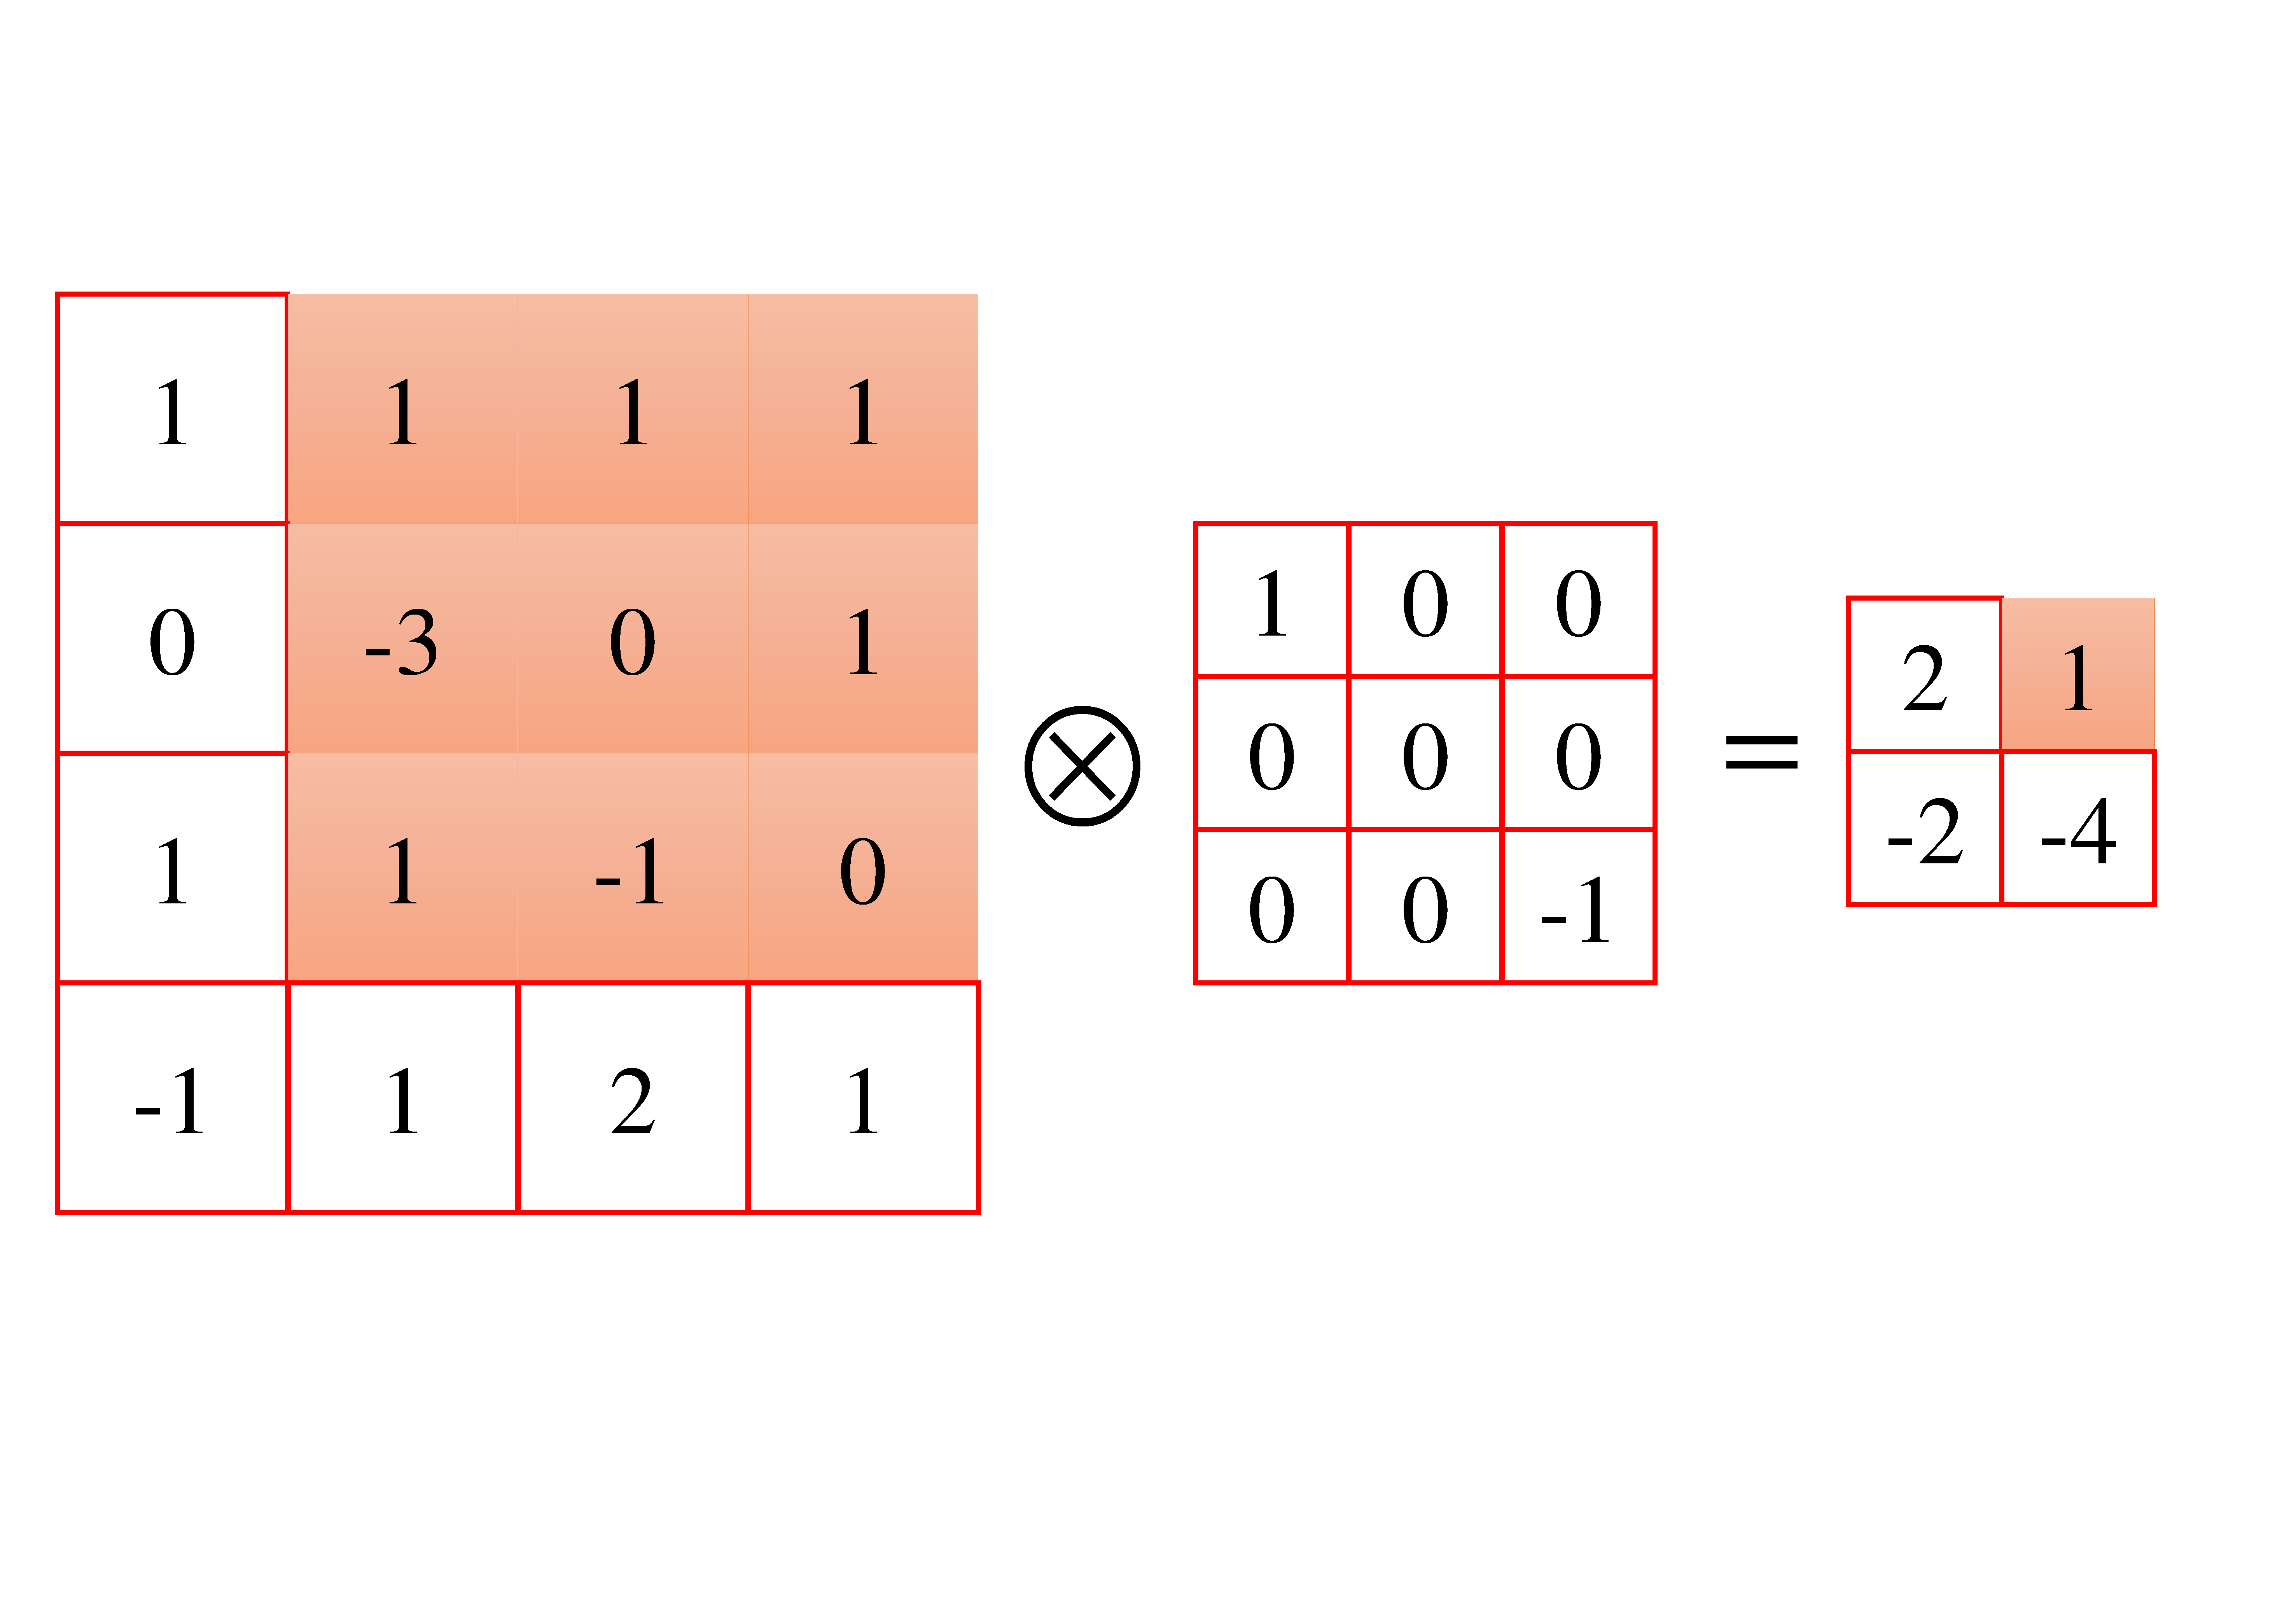
\includegraphics[width=0.7\linewidth]{figures/2dconv.pdf}
        \caption{二维卷积过程}
        \label{fig:2dconv}
    \end{figure}
    \item 池化层 \\
    池化层可以理解为下采样,减少输出特征的尺寸,能扩大感受野还能减少参数。最大池化和平均池化是最常见的两种方法。一般卷积层后会配合一个池化层,能进一步提取到有效的特征,保留主要特征并减少参数。
    \item 全连接层 \\
    无论说是一般的深度学习网络还是 CNN 这样稍微复杂的网络,全连接层都是关键所在。对于 MLP 这样的网络,那么就只有全连接层,可见全连接层的重要性。而对于卷积神经网络而言,全连接层就是将卷积层和池化层提取到的特征整合并输出预测结果。
\end{enumerate}

卷积层的提出极大地促进了计算机视觉领域的发展,AlexNet\cite{2012ImageNet} (5层卷积层、3层全连接层)在2012年的ImageNet视觉识别挑战赛中斩获冠军,可见CNN对于图像这样高级语义任务的巨大能力。此后,VGG\cite{simonyan2014very} 网络改进了 AlexNet 的网络,使得整个网络更深(19层),这使他成为了2014年 ImageNet 挑战赛的第一名。随着 VGG 的提出,人们开始倾向把网络加深,期望获得更好的识别效果。但实际上随着网络的逐渐加深,更深的网络难以训练,出现了因网络太深导致模型退化的问题,这是由于层数越深,训练误差越大,这与深度神经网络的初衷是背道而驰的,也不符合神经网络拟合任意复杂函数的理论。

但是众所周知的是,深度神经网络并没有消失在人们的视野里,这是由于残差网络 Resnet 的出现,这会在下一节进行具体介绍。
\subsection{残差网络 Resnet}
Kaiming He 等人借鉴了 Highway Network\cite{srivastava2015highway} 的跨层连接思想,并提出了赫赫有名的残差网络 Resnet\cite{he2016deep} ,较好地解决了当神经网络极深时模型失效无法训练的问题,并且在当时的 ImageNet 大赛上获得了第一名的好成绩。本文使用的神经辐射场的网络是基于残差模块设计的,因此接下来详细介绍残差网络的设计想法。

如图~\ref{fig:resnet}所示,经典的残差网络由多个残差模块组成,因此可以根据需求自行设计网络的深度。残差网络核心思想是使用了 shortcut 这一操作,即将输入传到输出作为输出的一部分,用公式表达就是$H(x) = F(x) + x$,当$H(x) = x$时为恒等映射,这里的$F(x)$就是需要学习的残差。这样的设计原理是,当深度学习网络极深的时候,由于训练误差较大,无法提取出更抽象的特征,那么此时有了这样的残差结构,就可以学习到一个恒等映射,至少还能保留前面提取出的特征。虽然学习一个恒等映射不是非常容易,不过由于 shortcut 这一操作使得只需让残差往0的方向去学习即可,这样也同时有效避免了梯度消失的问题。resnet 的出现是具有划时代的意义的,它解决了极深的神经网络难以训练的问题,通过有效地学习到恒等映射来保证当网络越来越深的时候所导致的模型退化性能衰退的情况。

本文的基础网络架构就是引入了 skip connection(或者是上述的 shortcut )的操作来将输入的特征往网络深处传送,以此来训练出一个高质量的深度学习网络,这样才能学习到细粒度的连续的神经辐射场。
,
\begin{figure}[t]
    \centering
    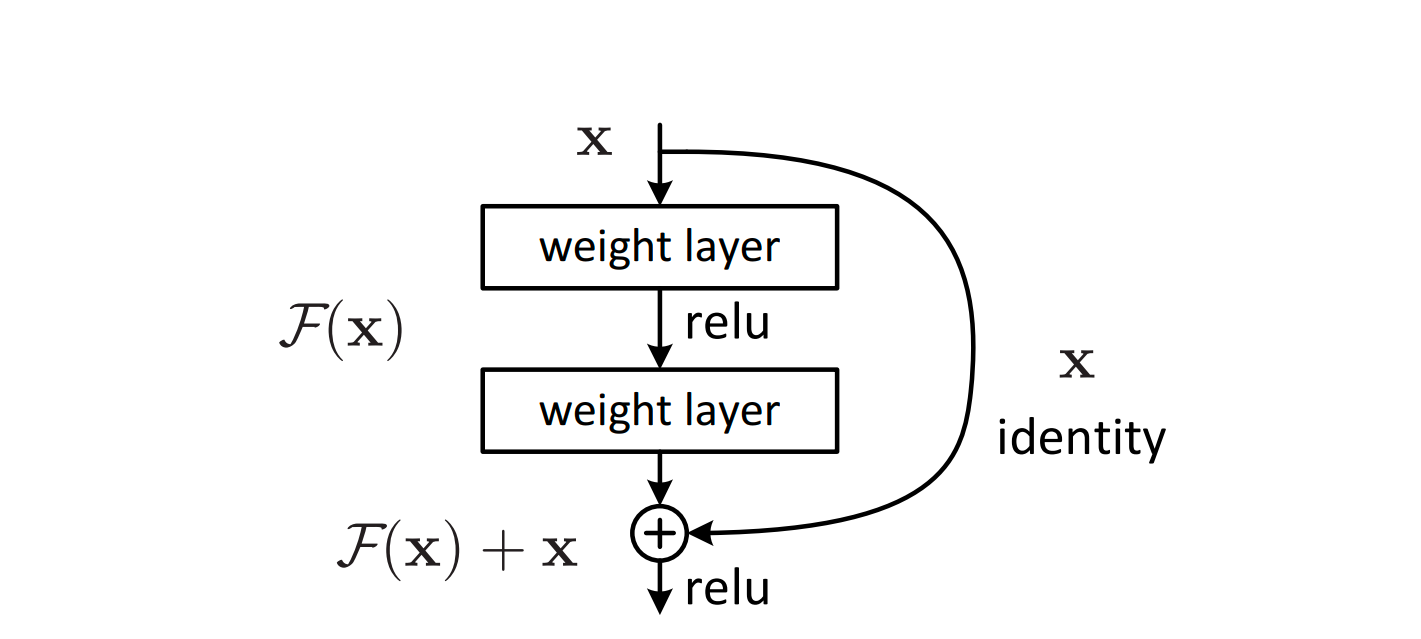
\includegraphics[width=0.7\linewidth]{figures/resnet.jpg}
    \caption{典型的残差结构}
    \label{fig:resnet}
\end{figure}

\section{查询表的加速方法}
在计算机科学中,查询表 (Lookup Table) 一般是一种简单的数组结构,通过简单的数组索引操作替代一些复杂的计算。一般来说,查询表的加速是很可观的,因为直接从内存中提取到相关数据往往要比复杂的计算快很多。

%一个经典的例子就是三角函数表。每次计算所需的正弦值在一些应用中可能会慢得无法忍受,为了避免这种情况,应用程序可以在刚开始的一段时间计算一定数量的角度的正弦值,譬如计算每个整数角度的正弦值,在后面的程序需要正弦值的时候,使用查找表从内存中提取临近角度的正弦值而不是使用数学公式进行计算。
一个典型的应用场景是自然对数表,在一些应用中,直接计算自然对数值是难以接受的,为了解决这一问题,可以提前将一些常用值的自然对数缓存在查询表中,在计算未知的对数值的时候,可以通过直接查询临近值的对数值而避免了复杂的数学计算,这大大加快了计算效率。

%一些折衷的方法是同时使用查找表和插值这样需要少许计算量的方法,这种方法对于两个预计算的值之间的部分能够提供更高的精度,这样稍微地增加了计算量但是大幅度地提高了应用程序所需的精度。根据预先计算的数值,这种方法在保持同样精度的前提下也减小了查找表的尺寸。

在一些细粒度的任务中,往往需要获得较高精度的查询结果,这时候就需要进行一些折衷,比如在使用查询表的同时结合插值的方法,通过略微增加计算量的方式增加了精度,同时也一定程度减少了查询表的尺寸。

%在图像处理中,查找表将索引号与输出值创建联系。颜色表作为一种普通的 LUT 是用来确定特定图像中每一像素所要显示的颜色和强度。

%另外需要注意的一个问题是,尽管查找表经常效率很高,但是如果所替换的计算相当简单的话就会得不偿失,这不仅仅因为从内存中提取结果需要更多的时间,而且因为它增大了所需的内存并且破坏了高速缓存。如果查找表太大,那么几乎每次访问查找表都会导致高速缓存缺失,这在处理器速度超过内存速度的时候愈发成为一个问题。
值得注意的是,虽然查询表的加速效率一般很高,但是通过查询表替换的计算方式过于简单,那么可能会出现从内存中提取数值的速度低于直接计算的速度,这样就得不偿失。

查询表实质是一种通过空间换时间的方式,但是实际应用中内存是有限的,因此必须要考虑查询表尺寸的问题。

%如何构建查找表有两个基本的约束条件,一个是可用内存的数量;不能构建一个超过能用内存空间的表格,尽管可以构建一个以查找速度为代价的基于磁盘的查找表。另外一个约束条件是初始计算查找表的时间——尽管这项工作不需要经常做,但是如果耗费的时间不可接受,那么也不适合使用查找表。

如图\ref{fig:justlookup}所示,以 justlookup\cite{lin2019justlookup} 为代表的工作拓宽了查询表的使用,justlookup 已经证明了对逐点网络可以去构建查询表来加速网络的前向传播并通过对近似特征再学习的策略来维持模型精度不损失,这一思想也可以应用到本文的模型加速上,通过查询表缓存网络参数,以此替换掉一些全连接层,这样可以少经过一些网络而直接通过查询表查询到中间层网络特征,从而加速前向传播。查询表技术在本文的具体应用详见下一章。

\begin{figure}[t]
    \centering
    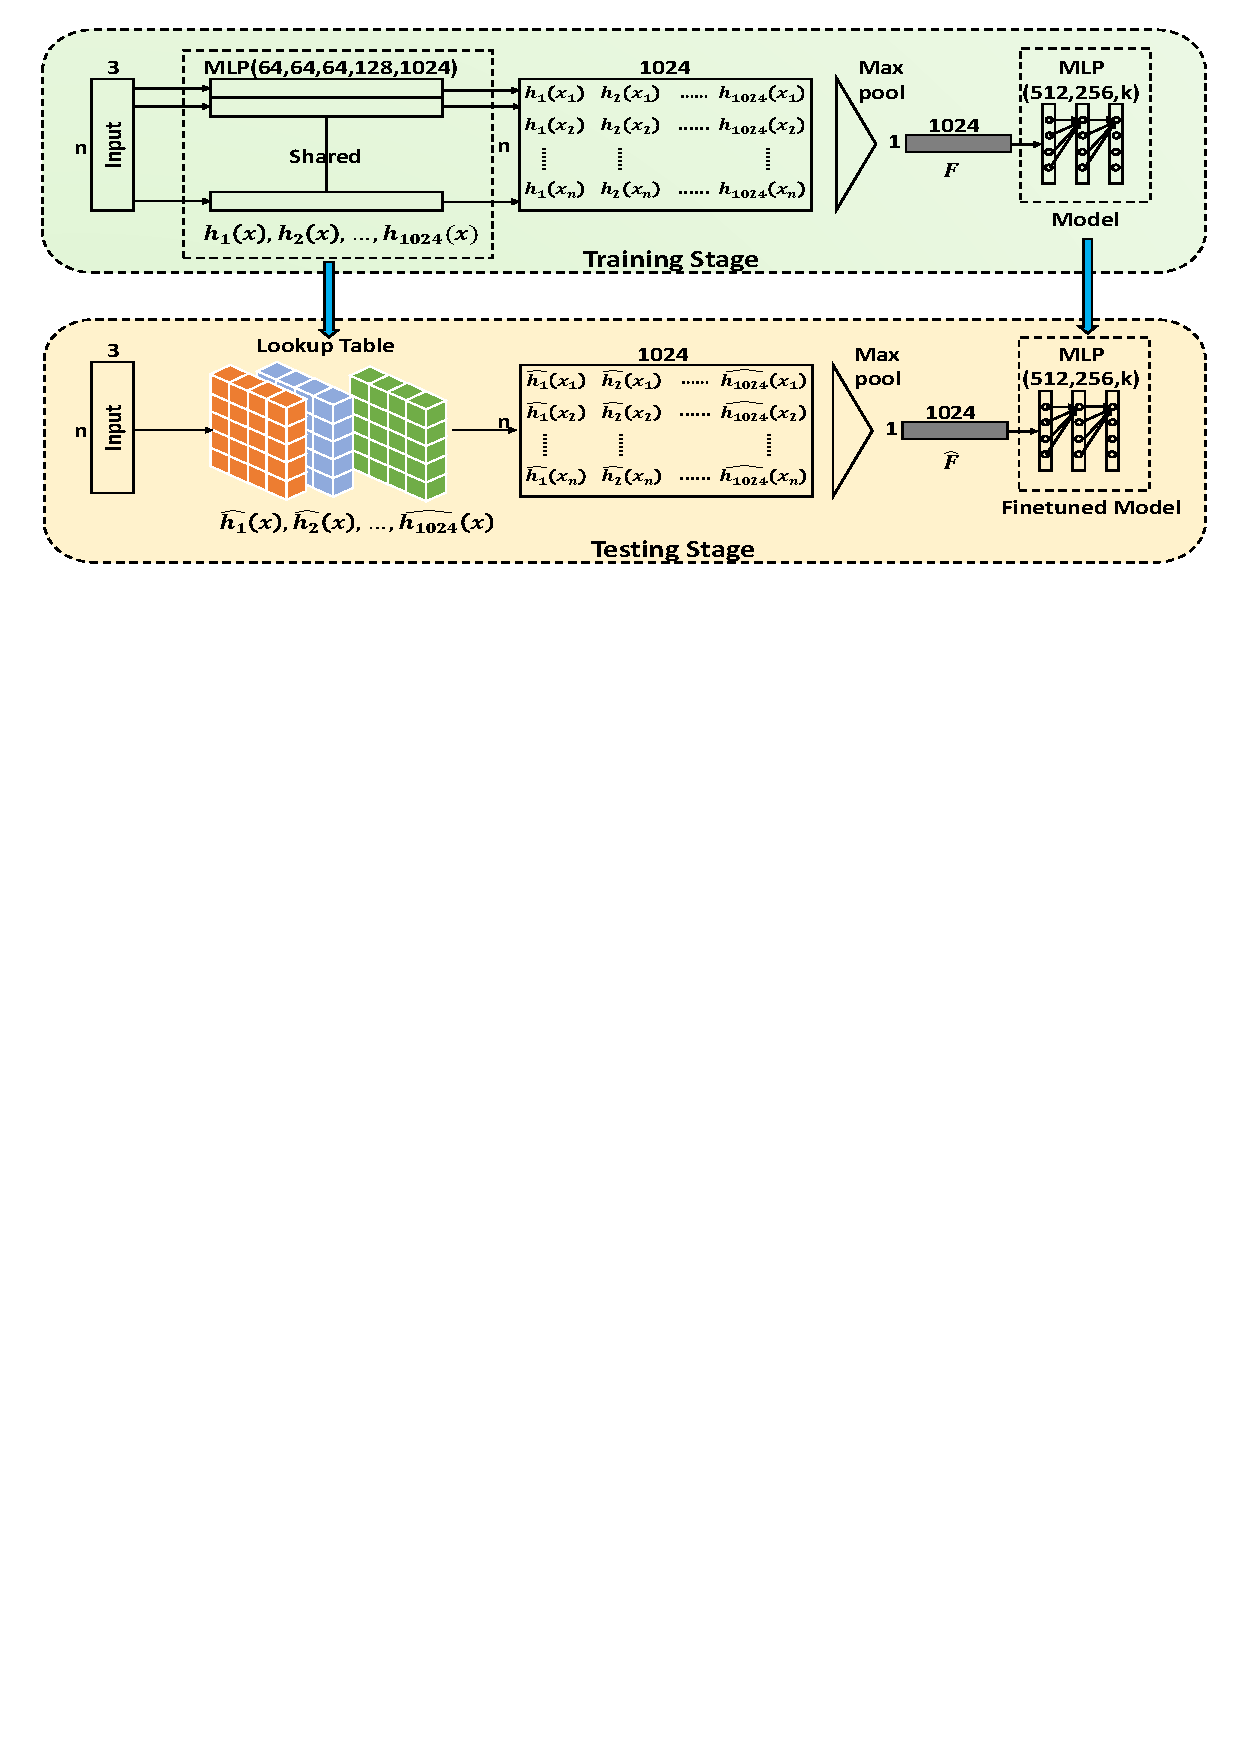
\includegraphics[width=0.9\linewidth]{figures/justlookup.pdf}
    \caption{查询表在逐点网络上的应用\cite{lin2019justlookup}}
    \label{fig:justlookup}
\end{figure}


\section{本章小结}
本章介绍了与本文研究技术相关的一些技术以及理论,包含用于描述 3D 形状的一些表示方法,以及与本文任务最相关的新视图合成和基于图像的渲染,还有关于深度学习的一些基础概念,这些都构成了本文方法的基础。最后介绍了关于查询表的加速方法,以及将其应用到含有逐点网络的前向传播上的经典方法,这一思路也成为了本文方法的根基,将在下一章节详细阐述本文的方法。

%     \cleardoublepage
%     % !TeX root = ../main.tex

\chapter{本文提出的方法}\label{citations}
上一章对本文研究相关的神经辐射场应用于新视图合成的相关原理和技术进行了概述。本文的研究始终围绕着“基于神经辐射场的新视图合成加速”这一框架展开。本章主要详细介绍本文的方法论部分,包含问题的定义,NeRF 的相关预备理论,以及本文提出的对 NeRF 加速的具体方法,最后是对本章的总结。

\section{问题定义}
本节将简要阐述本文所研究的问题定义。
首先本文的研究目标是基于移动端三维传感器采集的物体的不同视角的图像,快速渲染推理出新视角下的图像。要达到上述目标需要解决NeRF网络中如下的几个问题:
\begin{enumerate}
    \item 由于新视图合成是细粒度的渲染问题,NeRF 为了获取对渲染图象贡献较高的采样点,在训练和推理的过程中使用 coarse 网络和 fine 网络,通过 coarse 网络的输出来估计体密度随深度的变化分布,然后基于此分布进行二次采样并通过 fine 网络预测的颜色和体密度进行数值积分计算出 2D 图像对应像素的 RGB 值,这样两个网络的前向传播带来的开销是比较大的。
    \item NeRF 使用了深度学习网络,网络中较多的全连接层,尤其是该网络本质上是逐点网络,这对加速渲染过程来说也是能够优化的部分。
\end{enumerate}

\section{新视图合成的神经辐射场表示}
新视图合成的目的是基于已有的视角的图像,推理未知视角下的图像,现有的基于神经辐射场的体绘制方法已经可以合成较高质量的新视角图像。本节详细介绍神经辐射场 NeRF 的主要方法,包含神经辐射场的场景表示,基于神经辐射场的立体渲染,神经辐射场的优化三部分,由 NeRF 的方法论给本文提供一定的问题来源和理论支撑。

\begin{figure}[htbp]
    \centering
    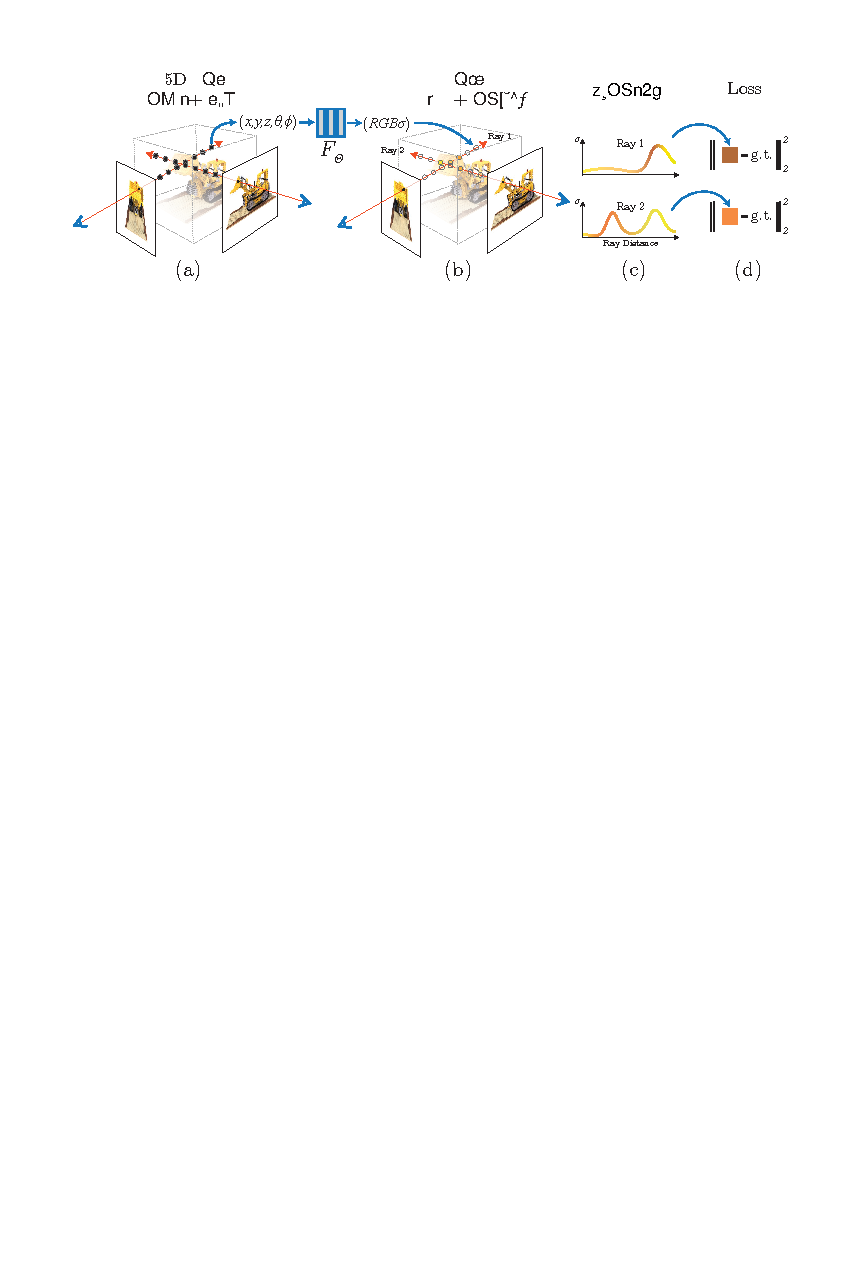
\includegraphics[width=0.95\linewidth]{figures/nerf_io.pdf}
    \caption{神经辐射场的场景表示和可微的渲染过程概况\cite{mildenhall2020nerf}。(a) 沿着相机光线采样 5D 坐标(位置和观测方向);(b) 将 (a) 中位置馈入 MLP 以生成颜色和体密度;(c) 将 (b) 中的这些输出使用立体渲染的方法合成相应的图像;(d) 此渲染过程是可微的,因此可以通过最小化合成的和 ground truth 观测图像之间的残差来优化场景表示}
    \label{fig:nerf_io}
\end{figure}

\subsection{神经辐射场的场景表示}
NeRF 的整体框架是使用 5D 的向量值函数来表示连续的场景,其中,输入是一个 3D 坐标$\displaystyle \symbf{x} = \left(x, y, z \right)$ 和 2D 的视角方向 $\displaystyle \left(\theta, \phi \right)$,输出是NeRF 的整体框架是使用 5D 的向量值函数来表示连续的场景,其中,输入是一个 3D 坐标$\displaystyle \symbf{x} = \left(x, y, z \right)$ 和 2D 的视角方向 $\displaystyle \left(\theta, \phi \right)$,输出是发出的颜色$\displaystyle \symbf{c} = \left(r, g, b \right)$和体密度$\displaystyle \sigma$。实际上,方向被表示为三维直角坐标系中的单位向量$\displaystyle \symbf{d}$。NeRF 通过 MLP 网络$\displaystyle F_{\Theta} : \left(\symbf{x}, \symbf{d} \right) \Rightarrow \left(\symbf{c}, \sigma \right)$ 来估计这个连续的 5D 场景表示,并优化网络权重 $\displaystyle \Theta$ ,建立起 5D 坐标到相应的体密度以及方向发出颜色的映射。

\subsection{基于神经辐射场的立体渲染}
NeRF 的 5D 神经辐射场将场景表示为空间内任意一点的体密度和定向发出的辐射,并且使用经典体积渲染的原理来渲染穿过场景的任何光线的颜色。体积密度$\displaystyle \sigma \left(\symbf{x} \right)$可以解释为一条光线在$\displaystyle \symbf{x}$的位置处终止于无穷小粒子的概率。相机光线$\displaystyle \symbf{r}\left(t \right) = \symbf{o} + t \symbf{d}$在近远界限分别为$\displaystyle t_n$和$\displaystyle t_f$时所对应的颜色的期望为:
\begin{equation}
    C \left(\symbf{r} \right) = \int_{t_n}^{t_f}T\left(t\right)\sigma\left(\symbf{r}\left(t\right)\right)\symbf{c}\left(\symbf{r}\left(t\right), \symbf{d}\right)dt, 
    \mbox{其中}T\left(t\right) = \exp \left(-\int_{t_n}^{t}\sigma\left(\symbf{r}\left(s\right)\right)ds\right).
\end{equation}
$\displaystyle T\left(t\right)$表示沿光线从$t_n$到$t$的累积透射率,即$t_n$到$t$光线没有碰到任何粒子的概率。从连续的神经辐射场中渲染一个视角需要估计通过所需虚拟相机的每个像素跟踪的相机射线的积分$\displaystyle C\left(\symbf{r}\right)$。

计算机是无法计算连续积分的,因此需要用到数值估计,利用求面积法来估计连续积分。 确定性求面积通常用于渲染离散体素网格,将有效地限制所表示的分辨率,因为 MLP 仅在固定的离散位置上查询。 相反,NeRF 使用分层抽样方法对$\displaystyle \left[t_n, t_f\right]$放入$N$个均匀分布的容器中,然后从每个容器中随机抽取一个样本:
\begin{equation}
    t_i \sim \mathcal{U} \left[t_n + \frac{i - 1}{N}\left(t_f - t_n\right), t_n + \frac{i}{N}\left(t_f - t_n\right) \right].
    \label{eq:uniform}
\end{equation}
虽然使用的是离散的样本集去估计积分,但是分层采样使的能表示连续的场景,这是因为它使的 MLP 在优化过程中在连续的位置进行评估。 最终是通过这些样本来估计$C(r)$。
\begin{equation}
    \hat{C}\left(\symbf{r}\right)=\sum_{i=1}^{N}T_i\left(1-\exp\left(-\sigma_i\delta_i\right)\right)\symbf{c}_i, \mbox{其中}T_i=\exp\left(-\sum_{j=1}^{i-1}\sigma_j\delta_j \right),
    \label{eq:getcolor}
\end{equation}
$\displaystyle \delta_i = t_{i + 1} - t_i$是相邻两个采样点的距离。这个函数对于计算$\displaystyle \hat{C}\left(\symbf{r}\right)$的一组$\displaystyle \left(\symbf{c}_i, \sigma_i\right)$值是可微的,使用 alpha 值 $\displaystyle \alpha_i = 1 - \exp \left(-\sigma_i\delta_i\right)$ 来简化成传统的 alpha 合成。 

\subsection{神经辐射场的优化}
上一节描述了将场景建模为神经辐射场并从该表示渲染新视图所必需的核心组件。 但是,NeRF注意到这些组件不足以实现更高质量。NeRF介绍了两项改进,以此表示高分辨率的复杂场景。 第一种是输入坐标的位置编码,可帮助MLP表示高频函数,第二种是分层采样过程,可让有效地采样此高频表示。

\subsubsection{位置编码}
尽管理论上神经网络可以拟合任何函数,但是 NeRF 发现直接向网络$\displaystyle F_{\Theta}$中输入$\displaystyle xyz\theta\phi$会使的渲染效果不是非常好,在颜色和几何的高频变化上表现的非常差。这与 Rahaman 等人\cite{rahaman2019spectral}最近的工作是一致的,该工作表明深度网络倾向于学习低频函数。他们还表明,在将输入传递到网络之前,使用高频函数将输入映射到更高维度的空间可以更好地拟合包含高频变化的数据。

在神经场景表示的背景下利用上述发现,把$\displaystyle F_{\Theta}$重构成一个由两个函数组成的复合函数$\displaystyle F_{\Theta} = F_{\Theta}^{\prime} \circ \gamma$,一个是学习的,另一个则是已知的,这能够明显地提升质量表现。$\displaystyle \gamma$建立了$\displaystyle \mathbb{R}$到更高维空间$\displaystyle \mathbb{R}^{2L}$的映射,$\displaystyle F_{\Theta}^{\prime}$仍是一个常规的 MLP。正式使用的编码函数如下:
\begin{equation}
    \gamma\left(p\right) = \left(\sin\left(2^{0}\pi p\right), \cos\left(2^{0}\pi p\right), \cdots, \sin\left(2^{L - 1}\pi p\right), \cos\left(2^{L - 1}\pi p\right)\right).
\end{equation}
$\displaystyle \gamma\left(\cdot\right)$函数被应用在$\displaystyle \symbf{x}$视角方向的单位向量$\displaystyle \symbf{d}$的每一个坐标值。

\subsubsection{分层体积采样}
接下来介绍一下 NeRF 中最核心的部分,分层体积采样。密集地评估沿着每条相机光线的$N$个查询点的神经辐射场网络的渲染策略效率低下:自由空间和对渲染图像无贡献的遮挡区域仍会被重复采样。 NeRF 从体绘制中的早期工作\cite{levoy1990efficient}中汲取灵感,并提出一种分层表示,通过按比例分配样本到最终渲染的预期效果来提高渲染效率。

NeRF 同时优化两个神经网络:一个是 coarse 网络,另一个是 fine 网络。首先使用分层采样采集一组有$N_c$个位置的样本,在这些位置使用公式~\ref{eq:uniform}和公式~\ref{eq:getcolor}来评估 coarse 网络。基于这个 coarse 网络的输出,就可以沿着每条光线对点进行更准确的采样,其中样本偏向体积的相关部分。为此,首先将~\ref{eq:getcolor}中的 coarse 网络$\displaystyle \hat{C}_{c} \left(\symbf{r}\right)$的alpha合成颜色重写为沿射线的所有采样颜色$\displaystyle c_i$的加权和:
\begin{equation}
    \hat{C}_{c}\left(\symbf{r}\right) = \sum_{i=1}^{N_c}w_{i}c_{i}, w_{i} = T_{i}\left(1 - \exp \left(-\sigma_{i}\delta_{i}\right)\right).
    \label{eq:weight}
\end{equation}
将上述权重进行归一化$\displaystyle \hat{w}_{i} = \frac{w_i}{\sum_{j=1}^{N_c}w_j}$可以生成一个沿着相机光线分段常数的概率密度函数。我们使用逆变换采样从该分布中采样第二组$\displaystyle N_f$个位置,最终使用公式~\ref{eq:getcolor}来计算最终沿着光线渲染的颜色,但是是使用所有$\displaystyle N_c + N_f$个采样点。

由于优化的是两个网络,因此整个 NeRF 的 loss 可以表示为:
\begin{equation}
    \mathcal{L} = \sum_{\symbf{r}\in \mathcal{R}}\left[\left\|\hat{C}_{c}\left(\symbf{r}\right) - C\left(\symbf{r}\right)\right\|_{2}^{2} + \left\|\hat{C}_{f}\left(\symbf{r}\right) - C\left(\symbf{r}\right)\right\|_{2}^{2} \right].
    \label{eq:nerf_loss}
\end{equation}
这个也是本文的动机 (motivation),通过构思,优化采样结构,使之可以减少训练一个网络,这是本文最核心的地方。

\section{基于神经辐射场的新视图合成加速方法}\label{method}
针对 NeRF 采用分层抽样这一做法,即同时优化 coarse 网络和 fine 网络,通过 coarse 网络的输出去估计公式~\ref{eq:weight}中的权重$\displaystyle w_i$的分布情况,生成一个分段常数的概率密度函数,这在 NeRF 中证明是能显著提升渲染质量的。但也正是由于增加了一个网络,那么在网络前向传播这一部分的开销增加了一倍,这在实际应用中是难以接受的。为此,我们将此问题看作是一个领域知识的优化的问题。我们的目标是无论是训练还是在测试过程中,只使用一个网络,这样理论上渲染一张新视图的时间会缩短一半。但是,在 NeRF 中证明了单纯地去减少一个网络势必会降低新视图渲染的质量,因此我们必须采取一定的方式去补偿减少一个网络带来的质量下降。接下来我们首先会介绍本文提出的一个最基本的加速优化模型;然后详细介绍该模型中的核心部分查询表的构建,其中包含网络架构和如何建立起索引的;

\subsection{模型综述}
本小节将详细介绍本文提出模型的设计方法和细节。
\begin{figure}[t]
    \centering
    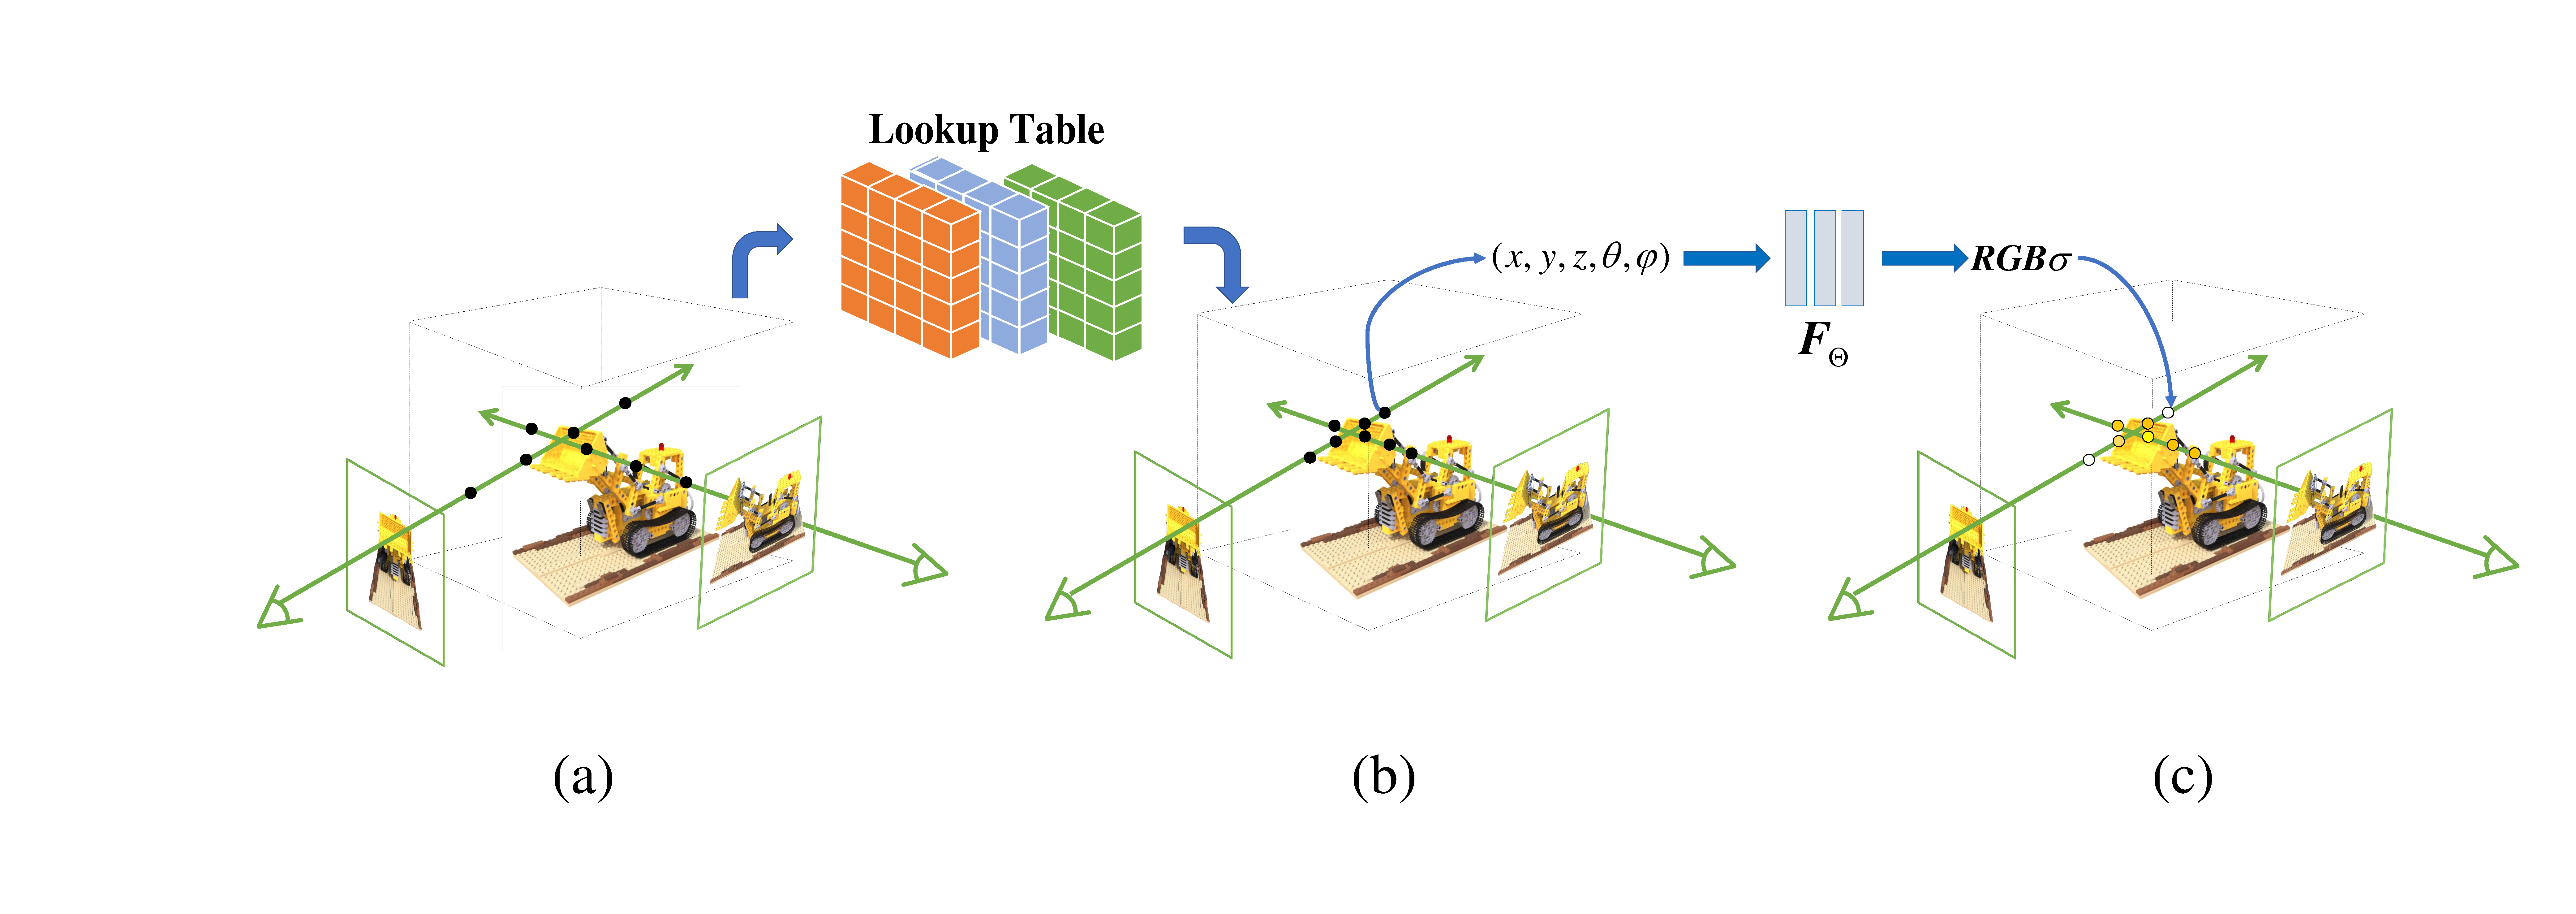
\includegraphics[width=0.95\textwidth, height=0.25\textheight]{figures/fnerf.pdf}
    \caption{神经辐射场的新视图合成的加速框架。(a) 沿着相机光线采样 5D 坐标(位置和观测方向);(b) 通过缓存的特征查询表找到采样点中距离表面最近的点,并在此点附近进行二次采样将 (c) 将 (b) 中位置和方向馈入 MLP 以生成颜色和体密度}
    \label{fig:fnerf}
\end{figure}
如图~\ref{fig:fnerf}所示,本文提出了基于神经辐射场的快速合成新视图的框架,为 NeRF 的推理过程进行提速。本文的框架一共包含三个步骤,第一步是网络裁剪,第二步是提取查询表,第三步是优化采样过程。

对于网络裁剪来说,由于 NeRF 是使用了 coarse 网络和 fine 网络来进行分层采样,为了操作方便,本文是去掉了 fine 网络,仅保留 coarse 网络,这显然会降低渲染的质量水平,因此还需要后面两个步骤的操作。对于提取查询表的过程,这里先简单理解为建立了一个立方体网格,将格点坐标输入到 NeRF 预训练好的网络中,根据体密度为正值这一条件筛选出合格的点的坐标,真正存的是网络中间层的特征,查询表表征物体的近似表面,具体的查询表的构建详见下一小节。对于第三步,我们实现采样值的优化是通过查询表完成的,过程的概况为首先将粗采样的采样点(均匀采样完成的)馈入查询表中,若发现光线上所有点均不在查询表内则忽略该条光线,下面是有交集的情况,沿着光线的方向找到相机光线上第一个在查询表内的点,以此点为中心,适当的区间长度进行二次均匀采样,这些采样点即最终的采样点,位于物体表面附近,对渲染贡献较大。之后将采样点馈入 NeRF 原有的网络框架中输出颜色和体密度,通过积分计算出像素的 RGB 值可以和 ground truth 计算出 loss 并反向传播优化整个网络,最后我们就获得了一个能快速合成新视图的网络框架。

\subsection{查询表的构建}
\begin{figure}[t]
    \centering
    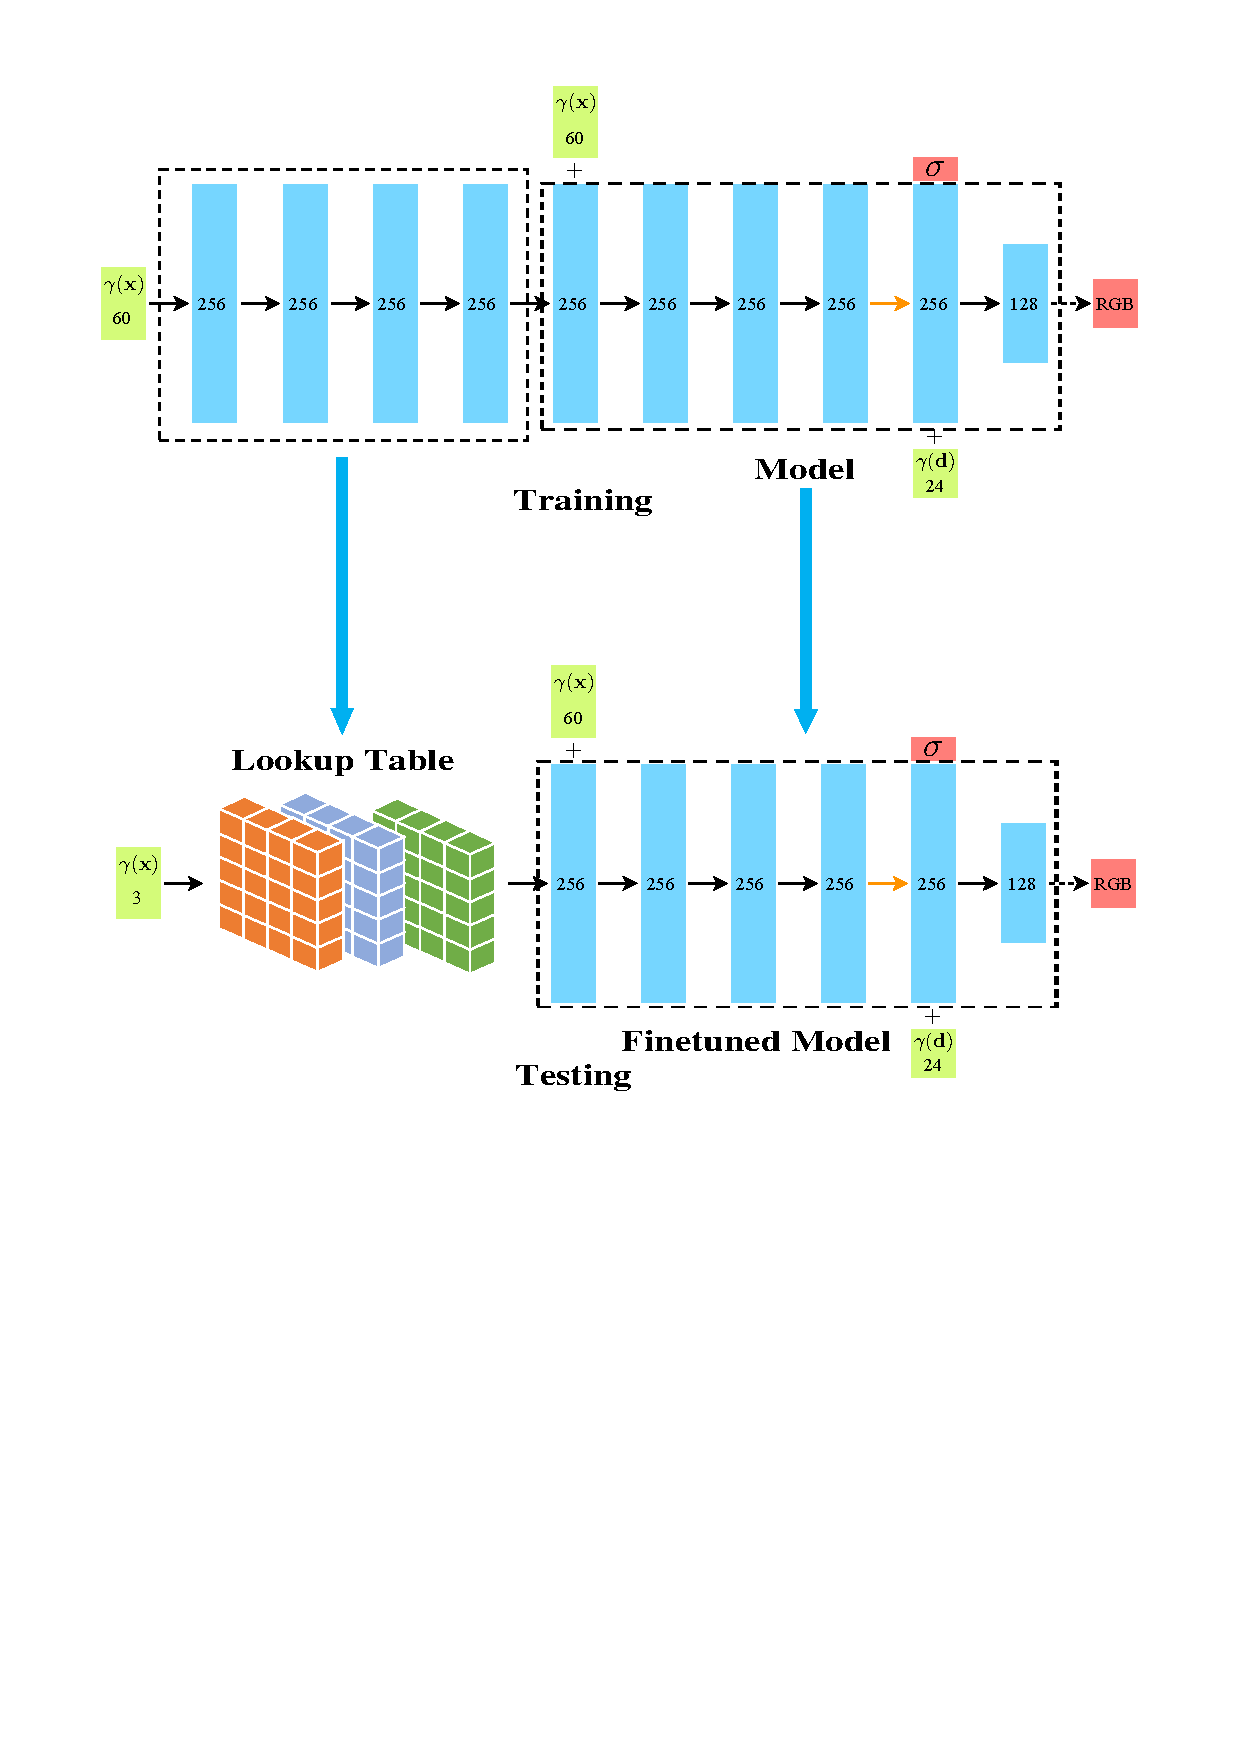
\includegraphics[width=0.95\textwidth]{figures/lookuptable.pdf}
    \caption{查询表的构建以及类似justlookup\cite{lin2019justlookup}的架构,通过缓存网络特征来进行加速,并通过重新训练的方法对近似的特征进行学习。}
    \label{fig:lookuptable}
\end{figure}

本节将详细介绍前一节中查询表的构建,主要介绍查询表的数据类型,获得方式,索引方法,以及如何压缩 NeRF 的网络。

如图~\ref{fig:lookuptable}所示,本文主要的构建方法是首先给采样点训练一个逐点网络,即使用 NeRF 的原网络进行预训练,将网络的前四层全连接层提取出来,我们可以得到一个逐点函数$\mathcal{G}$,类似justlookup\cite{lin2019justlookup},我们使用查询表技术并利用数组索引的方法能够快速地获得近似的函数$\hat{\mathcal{G}}$。

详细地,由前面的理论可知,我们可以用相机光线$\symbf{r}\left(t\right) = \symbf{o} + t \symbf{d}, t \in \left[t_n, t_f\right]$表示一组采样点的集合,为了使用方便,事先对光线的坐标范围进行尺度缩放,使的
$\forall t \in  \left[t_n, t_f\right], \symbf{r}\left(t\right) \in \left[-1, 1\right]^3$。

先忽略位置编码函数$\gamma\left(\cdot\right)$的影响,假设逐点网络输入的是三维坐标点,那么我们可以将上述的映射$\mathcal{G}$表示为$\mathcal{G}: \mathbb{R}^3 \Rightarrow \mathbb{R}^l$, 其中$l$在是第四层全连接网络输出变量的个数,在本文中$l = 256$。更具体地,$\mathcal{G}$是由四层 MLP 实现的,每一层的输出的数目分别是256,256,256,256。

为了学习$\mathcal{G}$,我们利用原网络剩下的部分记为 Model 。使用公式~\ref{eq:nerf_loss}中的均方误差联合优化这个端到端的网络,最终得到三元函数$\mathcal{G}$。一旦我们获得了$\mathcal{G}$,我们就可以通过构建一个查询表来获得近似的函数$\hat{\mathcal{G}}$。

显然,我们现在的最重要的一步是为$\mathcal{G}$构建查询表。为了方便,我们还是假设输入被缩放到一个固定大小的立方体$\mathcal{V}$里,其中$\mathcal{V} = \left[-1, 1\right]^3$。接着将$\mathcal{V}$分成规则的$M^3$个相等的体素块。那么每一个体素的边长则为$\Delta = \frac{2}{M}$。
% 那么因此立方体$\mathcal{V}$则被分成了:
% \begin{equation}
%     \mathcal{V} = \bigcup_{i,j,k}\left[i\Delta, \left(i + 1\right)\Delta\right] \times \left[j\Delta, \left(j + 1\right)\Delta\right] \times \left[k\Delta, \left(k + 1\right)\Delta\right], \mbox{其中} \left(i, j, k\right) \in \left[0, M\right]^3.
% \end{equation}

区别于justlookup\cite{lin2019justlookup},我们并没有采取$T\left[i\right]\left[j\right]\left[k\right] = \mathcal{G}\left(i\Delta, j\Delta, k\Delta\right), \left(i, j, k\right) \in \left[0, M\right]^3$,即存下所有格点所对应的特征,这样在 NeRF 这样细粒度的渲染工作中几乎是不可取的。实际中,我们需要使用 float32 的数据类型去存储,那么总内存开销就会达到$32M^{3}l bits$,以$l = 256, M = 256$为例,则需要$\SI{16}{GB}$的内存,随着查询表的边长$M$增加,内存是以三次方的速度在增长,这在实际操作中是不可行的。

\begin{figure}[b]
    \centering
    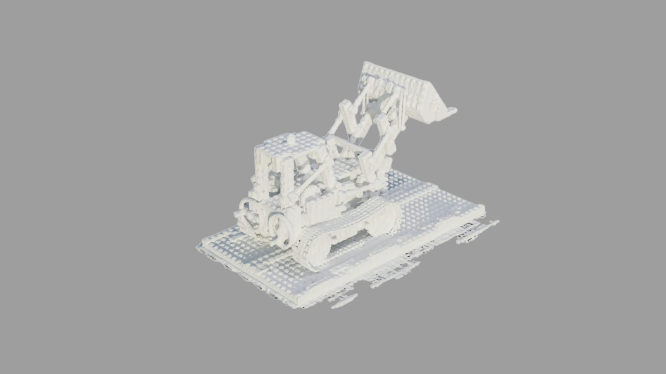
\includegraphics[width=0.95\textwidth]{figures/legomesh_gray_complete.png}
    \caption{使用 NeRF 网络(体密度 $> 0$)提取出的乐高的网格结构}
    \label{fig:lego_mesh}
\end{figure}

为此,我们必须采取相应的措施去压缩查询表。受 DeepSDF \cite{park2019deepsdf}的启发,在 DeepSDF 这篇工作中,可以通过输出的 SDF 值,利用 marching cubes 算法\cite{lorensen1987marching}重建物体的几何结构,类似地,我们知道 SDF 的物理含义是某一三维坐标点到物体表面的最短距离,负值表示在物体内部,正值表示在物体外部,零值则是物体表面;那么,NeRF 输出的体密度信息也有着相似的性质,体密度的物理含义是相机光线终止于某一点的概率,那么同样地,体密度为零值也可以表征物体的表面, 图~\ref{fig:lego_mesh}就是用 NeRF 模型提出乐高玩具的 mesh 结构。根据公式~\ref{eq:weight}可以看出当体密度为负值时权重$w_i$是负值是没有意义的,这也与 NeRF 的处理方式相同,NeRF 在体密度输出的时候使用了 ReLU 函数,因此我们可以认为负值的体密度对渲染的贡献可以忽略。那么结合上一节,如果我们可以将采样点约束在物体表面附近,那么将能获得更好的渲染效果,这可以补偿减少一个网络带来的质量下降的问题。

基于以上的分析,我们假设正值的体密度表征物体的内部,接下来就可以对原查询表进行压缩。我们的目标是只存$\mathcal{V}$中输出的体密度大于零的格点,这样可以大大减少内存的开销。

具体地,我们记从三维坐标点到输出体密度这一部分网络对应的函数为$\mathcal{Q}$,此时压缩后的查询表为:
\begin{equation}
    T_{shrinked} = \left\{
    \mathcal{G}\left(i\Delta, j\Delta, k\Delta\right) | \mathcal{Q}\left(i\Delta, j\Delta, k\Delta \right)  > 0, \left(i, j, k\right) \in \left[0, M\right]^3 
    \right\}.
\end{equation}
至此,我们获得了最终的查询表,由于此查询表是不规则的,或者可以认为是稀疏矩阵,因此索引此查询表也跟常规的方法不同,接下来将详细介绍经过压缩后的查询表的索引。

对于$ T_{shrinked}$ 的存的每一个格点$\left(i\Delta, j\Delta, j\Delta\right)$, 我们必须将每一个常规索引$\left(i, j, k\right)$ encode 到一个唯一值 code ,换句话说,我们的目标是使的$\mathcal{V}$中的任何一个格点对应的code都是不重样的。为此,我们可以使用以下的函数:
\begin{equation}
    \mathcal{E}\left(i, j, k\right) = i + j\cdot M + k\cdot M * M, \left(i, j, k\right) \in \left[0, M\right]^3,
\end{equation}

这个对索引的编码操作可以使得将$\mathcal{V}$中的所有格点都区分开。

接下来,我们将建立一个 code 到 $T_{shrinked}$的查询表$\mathcal{H}$,。具体的建立方式为,
\begin{enumerate}
    \item[a)] 首先建一个大小$size = M + M^2 + M^3$的查询表$\mathcal{H}$,使之能装下$\mathcal{V}$中所有格点;
    \item[b)] 按照$T_{shrinked}$对应的所有点的顺序,假设其中一个点对应的常规索引为$\left(i, j, k\right)$,该点在$T_{shrinked}$的位置为$index$对其使用 encode 操作得到$code = \mathcal{E}\left(i, j, k\right)$;
    \item[c)] 之后填充查询表$\mathcal{H}$,具体做法是$\mathcal{H}[code] = index$。
\end{enumerate}
严谨来说,非$T_{shrinked}$的点在索引时,其$code$ 可能会超过$T_{shrinked}$的索引范围,因此,我们必须处理此问题。具体做法是,在$T_{shrinked}$的最后面加一个哨兵,即增加一个$l$维的全零的向量,假设目前$T_{shrinked}$存了$S$个点对应的特征。而$\mathcal{H}$在初始化的时候,初始值都设置为$S-1$,即当$\left(i, j, k\right)$不在查询范围内时,其$code$可以通过$\mathcal{H}$映射到$S-1$,那么将获取$T_{shrinked}\left[S-1\right]$的值,从而得到一个鲁棒的索引过程。

至此,我们可以总结整个索引的过程。给定一个空间直角坐标系的三维坐标点$\left(x, y, z\right)$,首先通过下面式子计算其常规索引:
\begin{equation}
    \left(i, j, k\right) = \left(\left \lfloor \frac{x + 1}{\Delta} \right \rfloor, \left \lfloor \frac{y + 1}{\Delta} \right \rfloor, \left \lfloor \frac{z + 1}{\Delta} \right \rfloor\right),
\end{equation}

有了常规索引后,需要对其进行 encode ,得到 $code = \mathcal{E}\left(i, j, k\right)$,之后通过 $\mathcal{H}$ 查询到 $code$ 对应的在$T_{shrinked}$中的索引,则整个查询过程为:
\begin{equation}
    T\left[i \right]\left[j \right]\left[k \right] = T_{shrinked} \left[\mathcal{H}\left[\mathcal{E}\left(i, j, k\right) \right] \right].
\end{equation}

最终,如果我们提前缓存了$T$,则可以使用$T\left[i \right]\left[j \right]\left[k \right]$的值去估计$\hat{\mathcal{G}}\left(x, y, z\right)$,因此$\hat{\mathcal{G}}$的将是非常快的,它的开销只取决于访问内存的时间。

显然,我们直接将$\hat{\mathcal{G}}$馈入到经过训练的模型 $Model$中会使渲染效果下降的,因为$\hat{\mathcal{G}}$并不完全正确
等于$\mathcal{G}$,$\hat{\mathcal{G}}$仅仅是$\mathcal{G}$的一个近似。因此为了保持渲染质量不下降,我们在构建了查询表$T$后,需要基于$\hat{\mathcal{G}}$对$Model$进行再学习(或着叫微调),这一操作能显著提升渲染质量,在$M = 200$的时候甚至可以达到和原始 NeRF 质量相当的性能。图~\ref{fig:lookuptable}表征了$\mathcal{G}$是如何由我们的方法实现的。

\subsection{查询表与本文方法的结合}
我们在上一小节详尽地叙述了查询表的创建过程,包含是如何用查询表的构建,索引,压缩,还有通过近似$\mathcal{G}$来进行加速,通过再学习将损失的质量调回原 NeRF 水平。接下来,本节将详细介绍查询表的第二重加速功能:将查询表应用于 NeRF 的采样过程。

如果只是使用查询表去近似$\mathcal{G}$,那么这并没有完全展现出本文最核心的方法。实际上,在上一小节中,我们不止做了这么多工作。我们都知道,在查询表的构建过程中,本文是对查询表进行了压缩的操作,这表面上只是为了减少查询表内存开销,事实上我们还应用了 NeRF 体密度的特性。

由于我们是使用的体密度$\sigma > 0$这一阈值条件对$\mathcal{V}$中格点进行筛选,仅在$T_{shrinked}$中保留其体密度为正值的点所对应的特征(即$l$维向量),并且我们还在$T_{shrinked}$的最后放置了哨兵来表征没有查询到相应点的特征。

因此,我们可以合理地使用$\mathcal{H}$和$T_{shrinked}$这两个查询表对输入的点进行判断,显然如果可查询到,则该点在物体内部,否则不在物体内部。具体地,由于设置了哨兵,我们实际可以只使用索引转换查询表$\mathcal{H}$。对于任意的常规索引$\left(i, j, k\right) \in \left[-1, 1\right]^3$,计算$\mathcal{H}\left[\mathcal{E}\left(i, j, k\right)\right]$的查询结果,若结果为$S - 1$,则原世界坐标$\left(x, y, z\right)$则不在物体(场景)的内部,若结果不为$S - 1$,则在物体内部。

\begin{figure}[t]
    \centering
    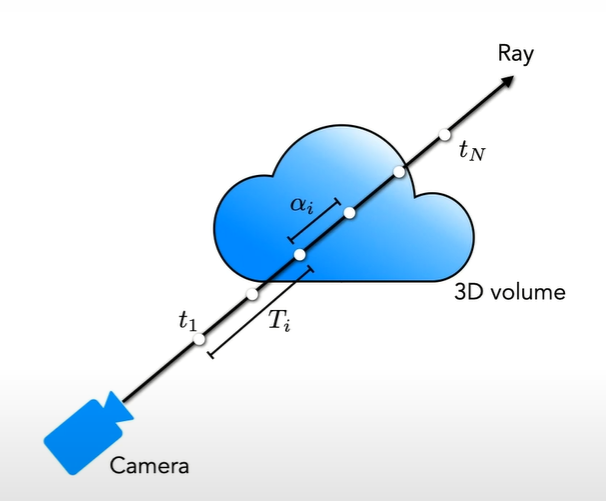
\includegraphics[width=0.95\textwidth]{figures/cloud.jpg}
    \caption{体绘制的采样示意图}
    \label{fig:cloud}
\end{figure}

有了以上的理论基础,接下来将详尽阐述是如何利用查询表进行采样优化以及加速的。

针对前面两节的概述,我们知道,NeRF 是采用分层抽样的方法,即同时优化 coarse 网络和 fine 网络,通过 coarse 网络的输出去估计公式~\ref{eq:weight}中的权重$\displaystyle w_i$的分布(概率密度函数),这是通过增加网络来提高渲染质量的方法。但同时也很显然,使用两个网络,那么时间开销会增加一倍。

为了加速 NeRF ,我们的目标是去掉一个网络,仅使用一个网络来进行优化和渲染,但是这势必会使的渲染质量下降。考虑到 NeRF 使用两个网络是为了优化采样点的选择,这一点启发了我们,如果使用上述的查询表将采样点约束到物体表面附近,那么渲染质量会比仅使用一个网络显著提升,通过实验证明本文的方法可以在几乎不损失渲染质量的情况下对 NeRF 的推理过程进行加速。下面是查询表是如何和本文方法进行融合的。

如图~\ref{fig:cloud}所示的是体绘制的采样示意图。假设相机光线为$\symbf{r}\left(t\right) = \symbf{o} + t \symbf{d}$,并在$\left[t_n, t_f\right]$的范围内均匀采样$N$个点,深度记为$t_{1}, t_{2}, \cdots, t_{N}$,这些深度是递增的,对应的点的世界坐标为$\symbf{r}\left(t_{1}\right), \symbf{r}\left(t_{2}\right), \cdots, \symbf{r}\left(t_{N}\right)$。分别计算这些点的常规索引,以及编码之后的 code,通过这些 code 去查询$\mathcal{H}$,得到一个长度为$N$的向量$vector$。之后按顺序对$vector$的每一个坐标值进行判断,若值均为$S - 1$,则说明该光线与物体没有交点,则采样点不需要优化,若存在值不为$S - 1$的,则说明光线和物体有交点,记第一个交点对应的深度值为$t_{mid}, mid \in \left\{1, 2, \cdots, N\right\}$。在有交点的情况下,我们需要重新设定采样区间长度为$L$,则新的采样区间为$\left[t_{mid} - L / 2, t_{mid} + L / 2\right]$,此区间能表征物体的表面附近,我们需要在此区间内重新均匀采样$N$个点,${t\prime}_{1}, {t\prime}_{2}, \cdots, {t\prime}_{N}$,然后就可以将$\symbf{r}\left(t\prime_{1}\right), \symbf{r}\left(t\prime_{2}\right), \cdots, \symbf{r}\left(t\prime_{N}\right)$这些采样点送入网络进行训练,最终实验证明使用了改进的采样方式,在我们减少一个网络的时候,可以保证渲染质量几乎不下降。

最终,我们通过缓存一个查询表,成功地在不损失精度的情况下减少了一个网络的开销,对渲染过程进行了加速,那么因此,本文方法对应的 loss 函数变为:
\begin{equation}
    \mathcal{L} = \sum_{\symbf{r}\in \mathcal{R}}\left[\left\|\hat{C}\left(\symbf{r}\right) - C\left(\symbf{r}\right)\right\|_{2}^{2} \right].
    \label{eq:nerf_loss}
\end{equation}

\section{本章小结}
本章首先介绍了本文所研究的问题定义。接着介绍了新视图合成任务中的神经辐射场表示方法,然后在此基础上详细地介绍了本文基于问题而提出的方法论,包含模型网络结构,查询表技术的引入与查询表的构建,以及如何把查询表应用到本文的方法中。

综上,本文借助查询表技术替换了一部分网络(逐点网络)参数,使得查询可以直接从内存(或缓存)中获取中间层的特征,这可以显著加速渲染过程;为了减少查询表的内存开销,同时也是为了与本文方法进行融合,我们对查询表进行了压缩的操作,具体是使用体密度$\sigma > 0$这一阈值条件去筛选位于物体内部的格点;本文的核心方法是减少 NeRF 的原始的两个网络的结构,我们仅采用一个网络进行训练和渲染,为了保证质量不下降,使用查询表判断原始采样点并第一个在物体内的点,并在此附近进行重新的均匀采样,可以补偿只用一个网络带来的质量下降;当然,最关键的一点是,将上述方法结合在一起时,由于查询表替换网络这一部分是用的近似特征,因此为了保证质量不下降,必须进行近似特征再学习。最终,通过本文的方法可以实现在几乎不损失精度的情形下对 NeRF 合成新视图进行加速。

\cleardoublepage

%     \cleardoublepage
%     \end{verbatim}
% \end{enumerate}

% 除上述文件外,
% 如无必要请勿修改其他重要文件,
% 如 \verb|sysuthesis-numeric.bst|(用于控制引文格式),
% \verb|sysuthesis.cls| (文档类,用于控制文档显示的样式)等。

% \section{编译文档}

% 可直接在命令行中使用 \texttt{latexmk} 命令,也可自己在编辑器中设置快捷键等。

% 为保证字体严格符合学校规定,建议终版文档在 Windows 平台上编译或在其他平台上安装 Windows 字体并修改\texttt{main.tex}中的文档选项,指定使用 Windows 字体。
% \begin{verbatim}
%     \documentclass[degree=doctor, fontset=windows]{sysuthesis}
% \end{verbatim}